
% YAML-metadata for possible future autogenerator
% ---
% language: finnish
% title_fi: Ajoneuvotietokoneen päivitysmahdollisuudet hakkuukoneessa
% title_en: Possibilities to upgrade Sunit Nero -embedded computer in Valmet 901 II -Harvester
% subtitle: ''
% author: Tomi Haapaniemi
% instructors_fi: Lehtori Keijo Länsikunnas
% instructors_en: Keijo Länsikunnas, Lecturer
% keywords_fi: Hakkuukone, ajoneuvotietokone
% keywords_en: harvester, in-vehicle computer
% ---

%\begin{document}


%----------------------------------------------------------------------------------------
%    Tiivistelmä
%----------------------------------------------------------------------------------------

\thispagestyle{tiivis}
\begin{tabular}{ | p{4,7cm} | p{10,3cm} |}
  \hline
  Tekijä \newline
  Otsikko \newline\newline
  Sivumäärä \newline
  Aika
  &
  \makeatletter
  \@author\newline
  \tiivistelmaotsikko\newline\newline
  \makeatother
  \pageref*{LastPage} sivua + \total{chapter} liitettä\newline %! if no appendices, risk to count total of chapter :D
  \pvm
  \\ \hline
  Tutkinto & \tutkinto
  \\ \hline
  Koulutusohjelma & \kohjelmatiivis
  \\ \hline
  Suuntautumisvaihtoehto & \suuntautumis
  \\ \hline
  Ohjaaja & \ohjaajat
  \\ \hline
  \multicolumn{2}{|p{15cm}|}{\begin{singlespacing}\vspace{-22pt}
  %Tämä on tiivistelmän ensimmäinen kappale. Tiivistelmän kappaleet loppuvat komentoon newline, jotta saadaan yksi tyhjä rivi aikaiseksi. \newline
  Insinöörityön tarkoituksena on selvittää 17 vuotta vanhan hakkuukoneen ajoneuvotietokoneen korvausmahdollisuudet. Työ tehtiin yksityiselle yrittäjälle. Loppukäyttäjän (hakkuukoneen kuljettajan) toiveesta korvaus tuli toteuttaa siten, että korvaavassa ajoneuvotietokoneessa toimisivat alkuperäisessä ajoneuvotietokoneessa käytetyt ohjelmistot. Työn tarkoituksena oli tuottaa lisää tietoa käytössä olevan hakkuukoneen käyttöiän ennusteesta koneen tietotekniikan osalta. Tavoitteena oli saada hakkuukoneeseen toimintakuntoinen, fyysisiltä ulkomitoiltaan yhteensopiva ajoneuvotietokone alkuperäisen tilalle. Insinöörityö rajattiin selvitykseksi kohtuullisen budjetin ja aikataulun rajoissa olevista päivitysmahdollisuuksista.\newline

  Haasteita työlle asetti hakkuukoneen sijainti metsässä 200 kilometrin päässä. Prosessin aikana käytiin alkuperäisen ajoneuvotietokoneen huoltojen yhteydessä hakkuukoneen luona yhteensä kolme kertaa. Lisäksi laitetta ja sen osia huollettiin etätyönä yrittäjän lähetettyä ne postitse, jolloin matka koneelle ei ollut välttämätön.\newline

  Työssä selvisi, että hakkuukoneen järjestelmät keskustelevat ajoneuvotietokoneen kanssa standardin RS-232-sarjaväylän kautta ja käytettävät ohjelmat on mahdollista saada toimimaan uudemmissa käyttöjärjestelmissä. Tämä mahdollistaa uudempien ajoneuvotietokoneiden tai fyysiseltä kestävyydeltään vastaavien tietokoneiden käytön hakkuukoneessa ilman muutoksia hakkuukoneen järjestelmiin. Uuden tietokoneen vaatimuksina oli lähinnä tarvittava olosuhteiden kesto ja tarvittavat liittimet. Hakkuukoneen järjestelmät vaativat kaksi sarjaporttiliitäntää, joilla kommunikointi hakkuukoneen ja ajoneuvotietokoneen välillä tapahtuu. Hakkuukoneen sähköjärjestelmä oli 24 V, mikä tuli ottaa huomioon tietokoneen sähkönsyöttöä pohdittaessa. \newline

  \end{singlespacing}} \\[14cm] \hline
  Avainsanat & \avainsanat
  \\ \hline
\end{tabular}
\clearpage

%----------------------------------------------------------------------------------------
%	ABSTRACT
%----------------------------------------------------------------------------------------

\pagestyle{abstract}
\begin{tabular}{ | p{4,7cm} | p{10,3cm} |}
  \hline
  Author \newline
  Title \newline
  Number of Pages \newline
  Date
  &
  \makeatletter4e
  \@author \newline
  \@title \newline
  \pageref*{LastPage} pages + \total{chapter} appendices \newline %! if no appendices, risk to count total of chapter :D
  \IfLanguageName {finnish} {\foreignlanguage{english}{\longdate\@date}} {\@date}
  \makeatother
  \\ \hline
  Degree & \metropoliadegree
  \\ \hline
  Degree Programme & \metropoliadegreeprogramme
  \\ \hline
  Specialisation option & \metropoliaspecialisation
  \\ \hline
  Instructor & \metropoliainstructors
  \\ \hline
  \multicolumn{2}{|p{15cm}|}{\begin{singlespacing}\vspace{-22pt}

The purpose of this thesis is to find out whether it is possible to replace the original computer in 17 y. old harvester with a newer computer so that there is no need to do any changes to the harvester's electronical systems. Therefore original communication protocols and controlling software must work in the new computer. User Experience of system with the new computer should be similar with the original computer.\newline

This thesis was done for a private entrepreneur and the results are intended to provide additional information about the life expectation of harvester from the viewpoint of computer systems. The original goal of the thesis was to produce a drop in -replacement computer for the original systems. Thesis is now  a report about the possibility to upgrade the original system with reasonable budget and time.\newline

The location of the harvester, which was approx. 30 km to forest from the Orivesi city center set some challenges for the thesis. Distance to Orivesi is approx. 200 kilometres from my home at Kirkkonummi. Harvester was visited total of three times. All visits took place after maintenance of the harvester's original computer. In addition the entrepreneur sent some parts for maintenance by mail so that a visit to Orivesi wasn't necessary.\newline

Result of the thesis is that all required communication with harvester is through standard RS-232 serial bus. All required software was proven to work in newer operating systems which allows the possible new system to be selected from a broader range of availabe rugged computer models without any modifications to harvester's electronical systems. \newline

Requirements for a new computer are durability in existing conditions and availability of required connectors. The harvester's systems require two serial port connections for communication between harverter's systems and vehicle computer. The harvester's electrical system is 24V DC, which must be taken into account when selecting the computer's power supply.


  \end{singlespacing}} \\[14cm] \hline
  Keywords & \metropoliakeywords
  \\ \hline
\end{tabular}
\clearpage

%----------------------------------------------------------------------------------------
%	Acknowledgement ?
%----------------------------------------------------------------------------------------
%\chapter*{Acknowledgement}
%Thanks to my cat
%\clearpage

%----------------------------------------------------------------------------------------
%	TABLE OF CONTENTS
%----------------------------------------------------------------------------------------

\makeevenhead{plain}{}{}{}
\makeoddhead{plain}{}{}{}
\pagestyle{empty} %remove page number in toc (if longer than 2 pages)
\tableofcontents*
\pagestyle{empty} %remove page number in toc (if longer than 1 pages)
\clearpage
\pagestyle{plain}

%list of figure, tables comes here...


%----------------------------------------------------------------------------------------
%    Lyhenteet / Abbreviation
%----------------------------------------------------------------------------------------

\pagestyle{empty}
\setlength{\parskip}{1cm}
\IfLanguageName {finnish} {
  \chapter*{Lyhenteet ja käsitteet}
  \cftaddtitleline{toc}{chapter}{Lyhenteet ja käsitteet}{}
} {
  \chapter*{Abbreviation}
  \cftaddtitleline{toc}{chapter}{Abbreviation}{}
}
\begin{table}[h]
\setlength{\tabcolsep}{8pt}
\renewcommand{\arraystretch}{2}
\begin{tabular}{l p{12cm}}
x86 & Yleisnimitys Intelin vuonna 1987 julkaisemalle CISC-prosessorikäskykannalle. Työssä x86:lla viitataan myös 80386:ssa käytössä olleeseen ja myöhempiin 32-bittisiin käskykannan versioihin.\\
PS/2 & Sarjaväyläinen, 7 IBM PS/2-koneessa ollut liitäntäprotokolla, joka yleistyi PC-koneiden standardiliitännäksi näppäimistölle ja hiirelle ennen USB-protokollaa.\\
RS232 & Alun perin vuonna 1962 esitelty asynkroninen sarjaliitäntäprotokolla, joka oli ennen USB-liitännän yleistymistä yleisin PC-koneiden oheislaitteiden liitäntäväylä.\\
USB & Universal Serial BUS, vuonna 1996 esitelty sarjaväyläinen liitäntä oheislaitteiden liitäntään.\\
IDE/PATA & Integrated Drive Electronics (Parallel AT Attachments), kiintolevyjen ja optisten asemien liittämiseen tarkoitettu 16-bittinen rinnakkainen liitäntäväylä vuodelta 1986.\\
CAN & Controller Area Network, vikasietoinen, differentiaalinen kaksijohtoinen automaatioväylä, jossa liikenne lähetetään priorisoituina sanomina, vuodelta 1986.\\
Apteeraus & Puun rungon jako eri puutavaralajeiksi mitta- ja laatuvaatimukset huomioiden.\\
GPS & Global Positioning System, maapalloa kiertäviin satelliitteihin perustuva paikannusjärjestelmä.\\
DPGS & Differential GPS, DGPS:ssä tarkennetaan sijaintitietoa käyttämällä apuna kiinteiden maa-asemien mittaamaa ja välittämää alueellista paikannusvirhettä.\\
Hypervisor & Järjestelmä tai ohjelmisto, joka hallitsee ja suorittaa virtuaalikoneita.\\
%
%OMG & Oh my god\\
%WTF & What the F\\
%TL;DR & Too long, didn't read\\
\end{tabular}
\end{table}

\newpage

%page number always on top right; also for chapter "title" page
\pagestyle{plain}
\makeevenhead{plain}{}{}{\thepage}
\makeoddhead{plain}{}{}{\thepage}

\setcounter{page}{1} %page 1 should be Introduction
\ClearWallPaper
%----------------------------------------------------------------------------------------
%	CONTENT
%----------------------------------------------------------------------------------------

\chapter{Johdanto}
Tietokoneiden käyttöikä on varsinkin vaativissa kohteissa rajallinen. Kun järjestelmät vanhenevat, huollon tarve lisääntyy, mutta varaosien saatavuus vähenee. Viimein voi tulla eteen piste, jossa ainoa mahdollinen vaihtoehto on korvata vanha järjestelmä uudella. Tämä saattaa vaatia suuriakin muutostöitä myös järjestelmää käyttäviin laitteisiin, ja siten usein on järkevämpää vaihtaa koko kohde kuin vaihtaa kohteen järjestelmät.

Insinöörityön tarkoituksena on vuonna 1998 valmistetun hakkuukoneen ajoneuvotietokoneen päivitysmahdollisuuksien tutkiminen. Alkuperäisessä, myös vuodelta 1998 olevassa ajoneuvotietokoneessa on alkanut näkyä ikääntymisen merkkejä. Laitteen komponentit rikkoutuvat yksitellen, ja se ylikuumenee etenkin kesäisin siten, että käyttöaika on vain pari tuntia kerrallaan. Osien saatavuus näin vanhaan tietokoneeseen alkaa luonnollisesti olla heikkoa.

Insinöörityö pyrkii selvittämään hakkuukoneen ja ajoneuvotietokoneen väliset liitännät ja ajoneuvotietokoneen ohjelmistot ja etsimään mahdolliset korvaavat ratkaisut. Tarkoituksena ja loppukäyttäjän (hakkuukoneen kuljettajan) toiveena oli, että korvaava järjestelmä vaatisi mahdollisimman vähän muutoksia hakkuukoneeseen ja olisi hakkuukoneen kuljettajalle toiminnallisuudeltaan vastaava kuin alkuperäinen järjestelmä.

Haasteita työlle tuovat huollettavan hakkuukoneen sijainti yli 200 kilometrin päässä ja alkuperäisten ohjelmien mahdollisesti asettamat vaatimukset. Lisäksi on huomioitava hakkuukoneen käyttöympäristö, joka asettaa ajoneuvotietokoneelle erityisiä vaatimuksia pölyn siedon, lämpötilan muutosten ja tärinän keston suhteen. Lähtötilanteessa käytetyistä alkuperäisestä järjestelmistä ei ole lainkaan tietoja, eikä tiedetä, miten ja mitä käyttöjärjestelmiä käyttäen järjestelmä on toteutettu.

\newpage

\chapter{Nykyinen järjestelmä}

\subsubsection{VALMET 901 II -hakkuukone}
Hakkuukoneet eli motot (monitoimikoneet) ovat metsätraktoreita, joiden tehtävänä ovat hakkuun kaikki työvaiheet. Hakkuukoneet sisältävät tietokoneohjatut mittalaitteet, joilla puiden katkonta ja mittaus saadaan hoidettua tarkasti.

Työn kohteena oleva hakkuukone on kuvassa \ref{hakkuukone} oleva, nelipyöräinen Valmet 901 II vuosimallia 1998. Kone on otettu käyttöön joulukuussa 1998. Värityksenä on Valmetin vanhempi punamusta-väritys. Valmet 901 on Valmetin senaikaisen malliston pienin hakkuukone, ja se tarkoitettu ensisijaisesti harvennushakkuisiin. Alkuperäinen hakkuupää on jälkikäteen vaihdettu toiseksi, jolloin myös apteeraukseen käytettävä ohjelmisto vaihtui. Hakkuukoneen alkuperäinen teleskooppipuomisto on vaihdettu liikeratapuomiksi.
\newline

\begin{figure}[H]
\centering
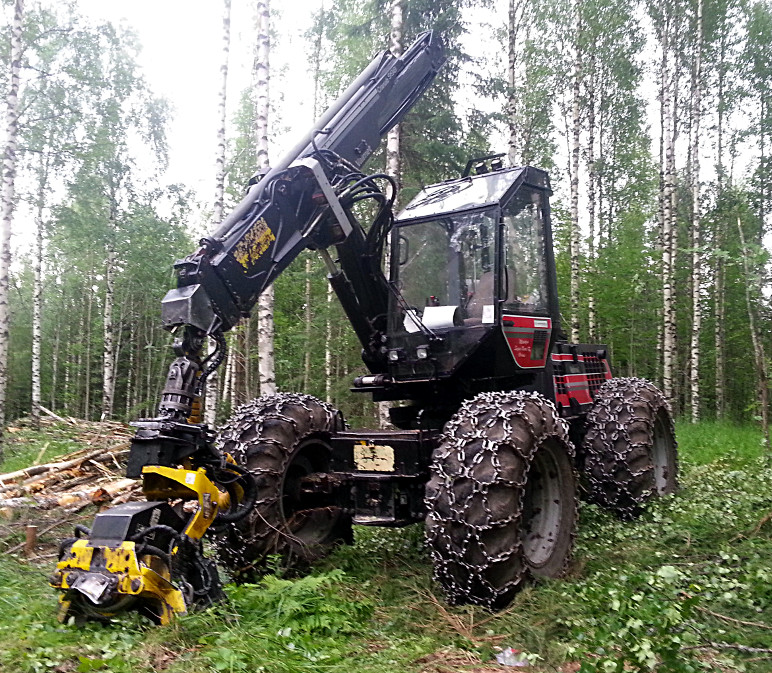
\includegraphics[width=0.700\textwidth]{moto_2.jpg}
\caption{Valmet 901 II -hakkuukone.}
\label{hakkuukone}
\end{figure}

\subsubsection{Motomit-mittalaite}
Työn kohteena olevaan hakkuukoneeseen on jälkiasennettu Motomit-IT-mittalaite, joka on korvannut hakkuukoneen alkuperäiset mittalaitteet ja ohjelmiston. Motomit IT tukee StanForD-standardin mukaista apteerausohjeiden tiedonsiirtoa. Se hoitaa sisäisen kommunikaation CAN-väylää pitkin. Kommunikaatiossa alkuperäisen ajoneuvotietokoneen kanssa käytetään RS232-väylää ja MotomitPC-ohjelmistoa kuvassa \ref{motomit:modulikaavio} näkyvällä tavalla. \citep{motomit:esite}
\newline

\begin{figure}[H]
\centering
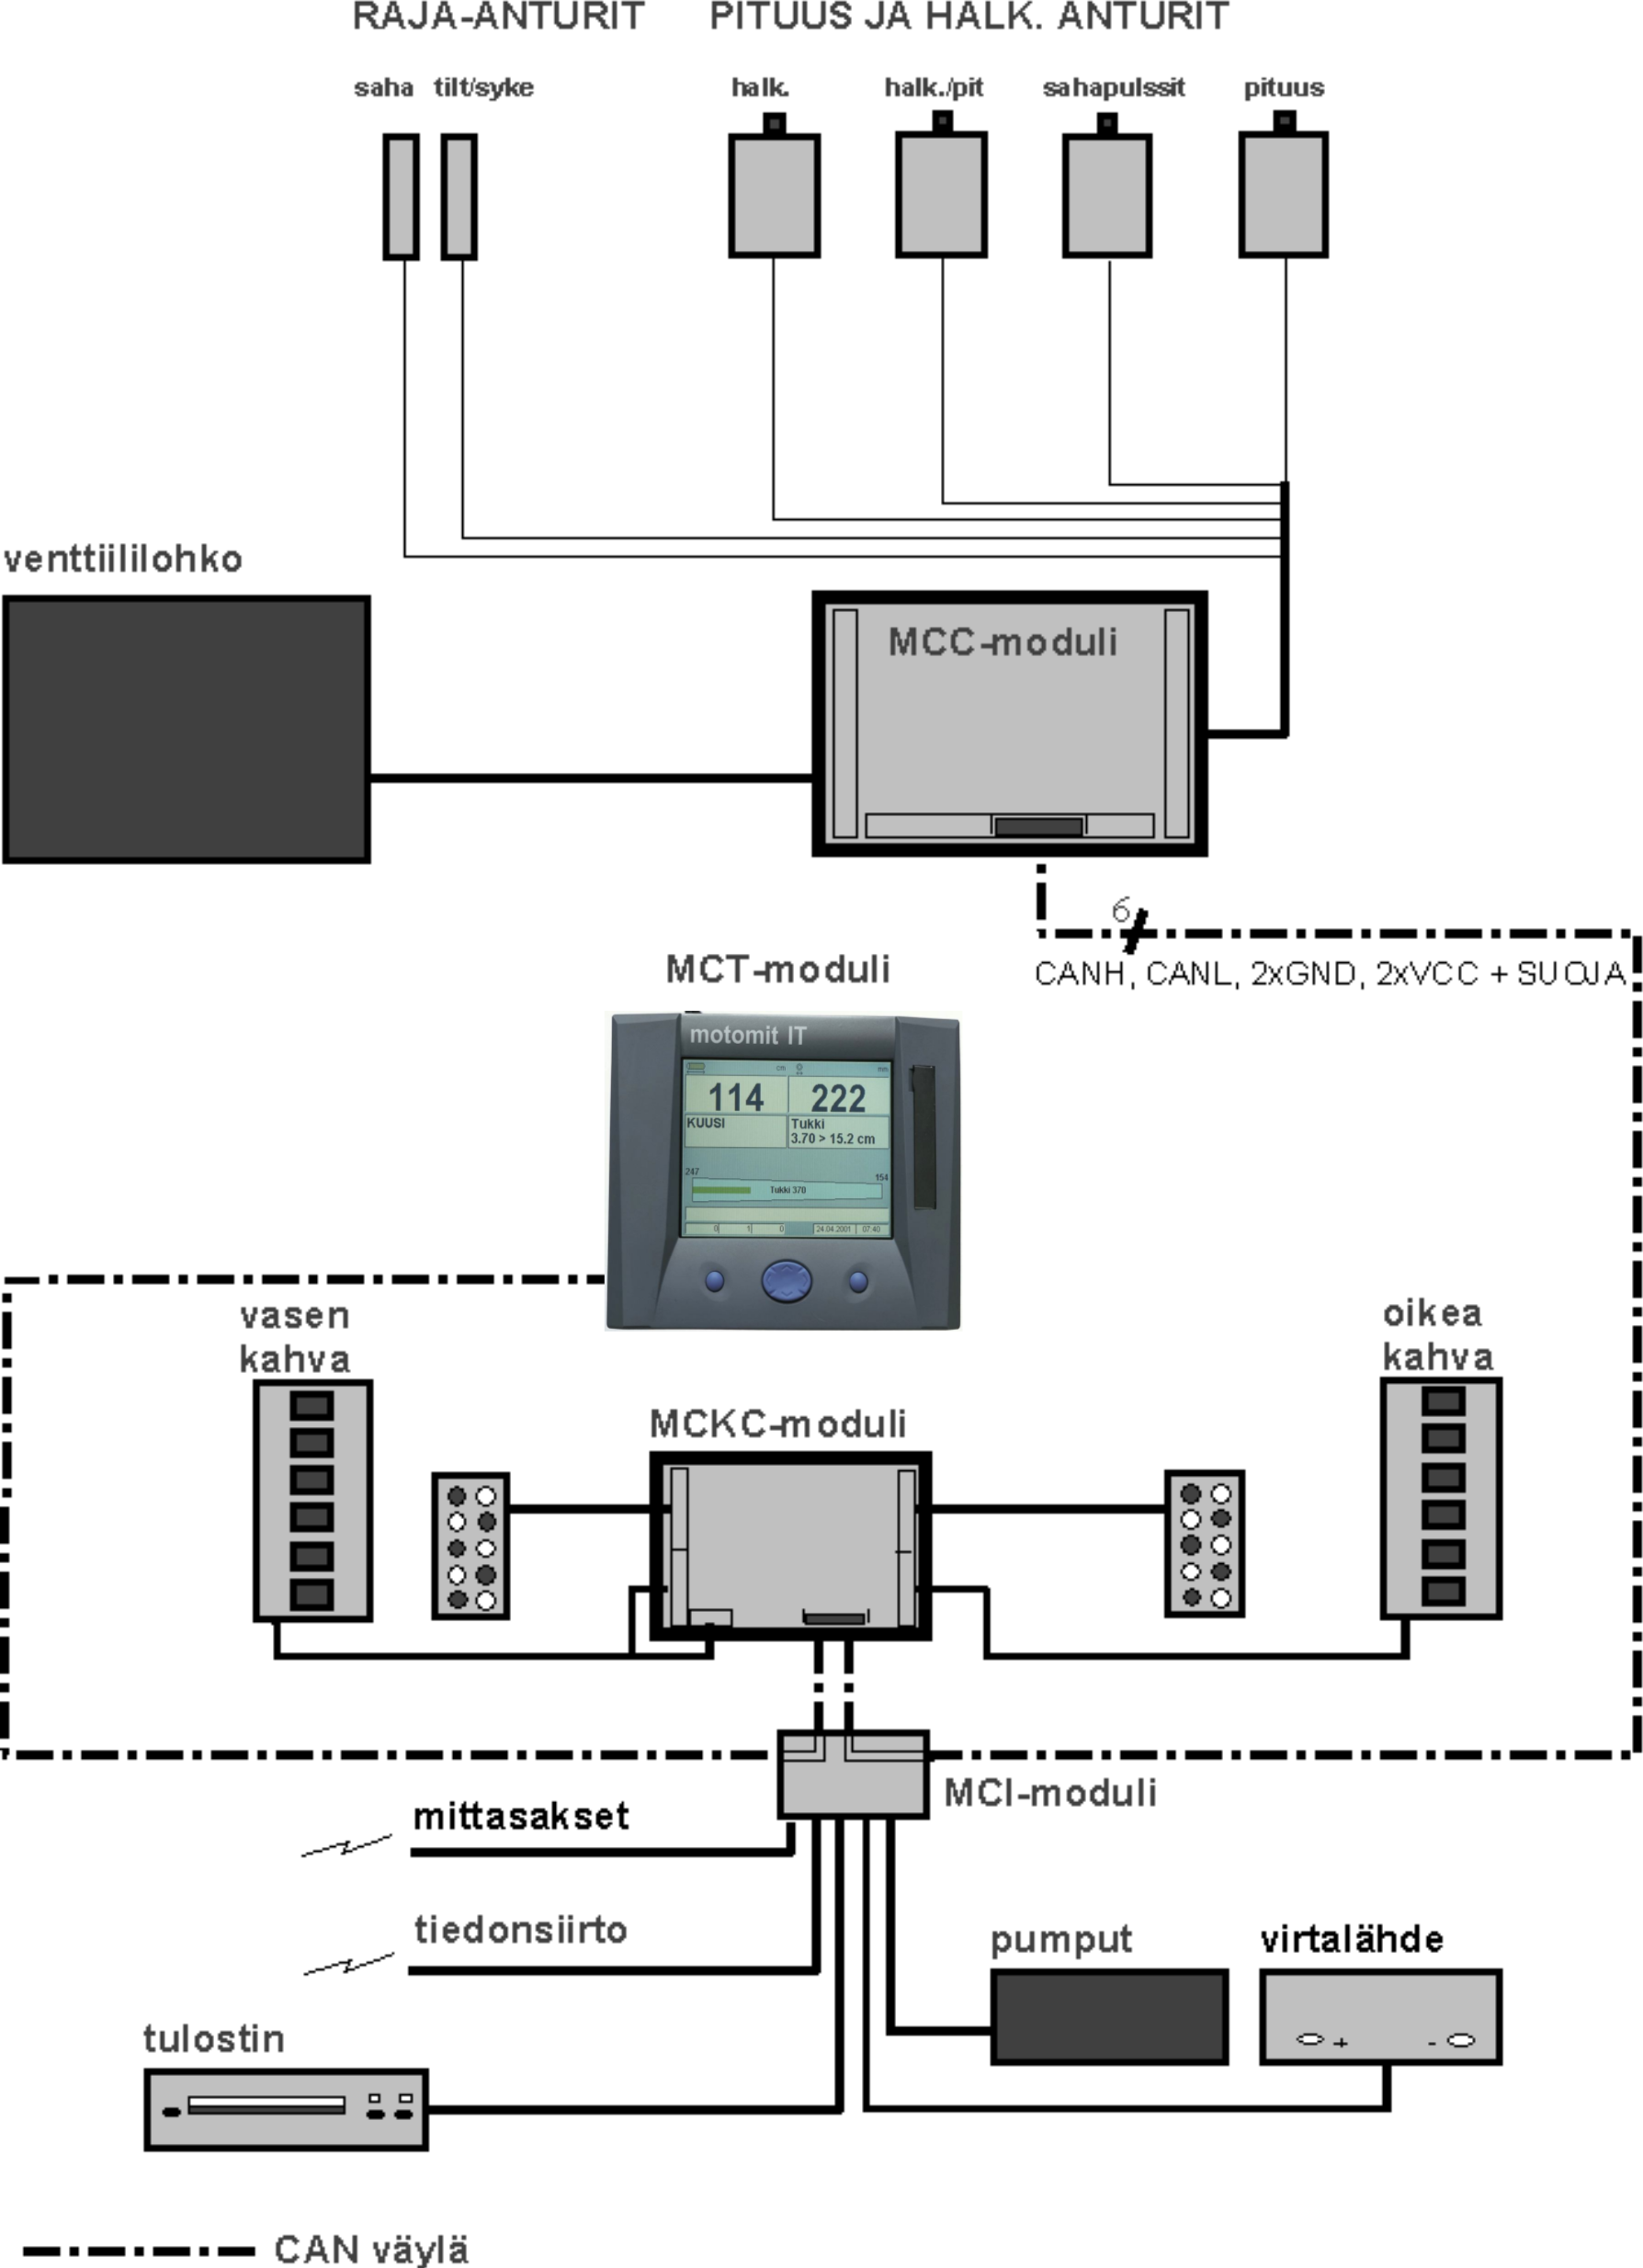
\includegraphics[width=0.700\textwidth]{motomit_kaavio.png}
\caption{Motomit IT:n moduulikaavio \cite{motomit:manual}.}
\label{motomit:modulikaavio}
\end{figure}
\newpage

Motomit PC (kuva \ref{motomit:kuvankaappaus}) on Motomit IT:n Windows-pohjainen näyttö- ja hallintaohjelmisto Motomit IT-järjestelmälle. Se kommunikoi Motomit IT:n MCI-moduulin (Mitron CAN Interface) kanssa RS-232-sarjaväylän avulla. \citep{motomit:esite}
\newline
\begin{figure}[H]
\centering
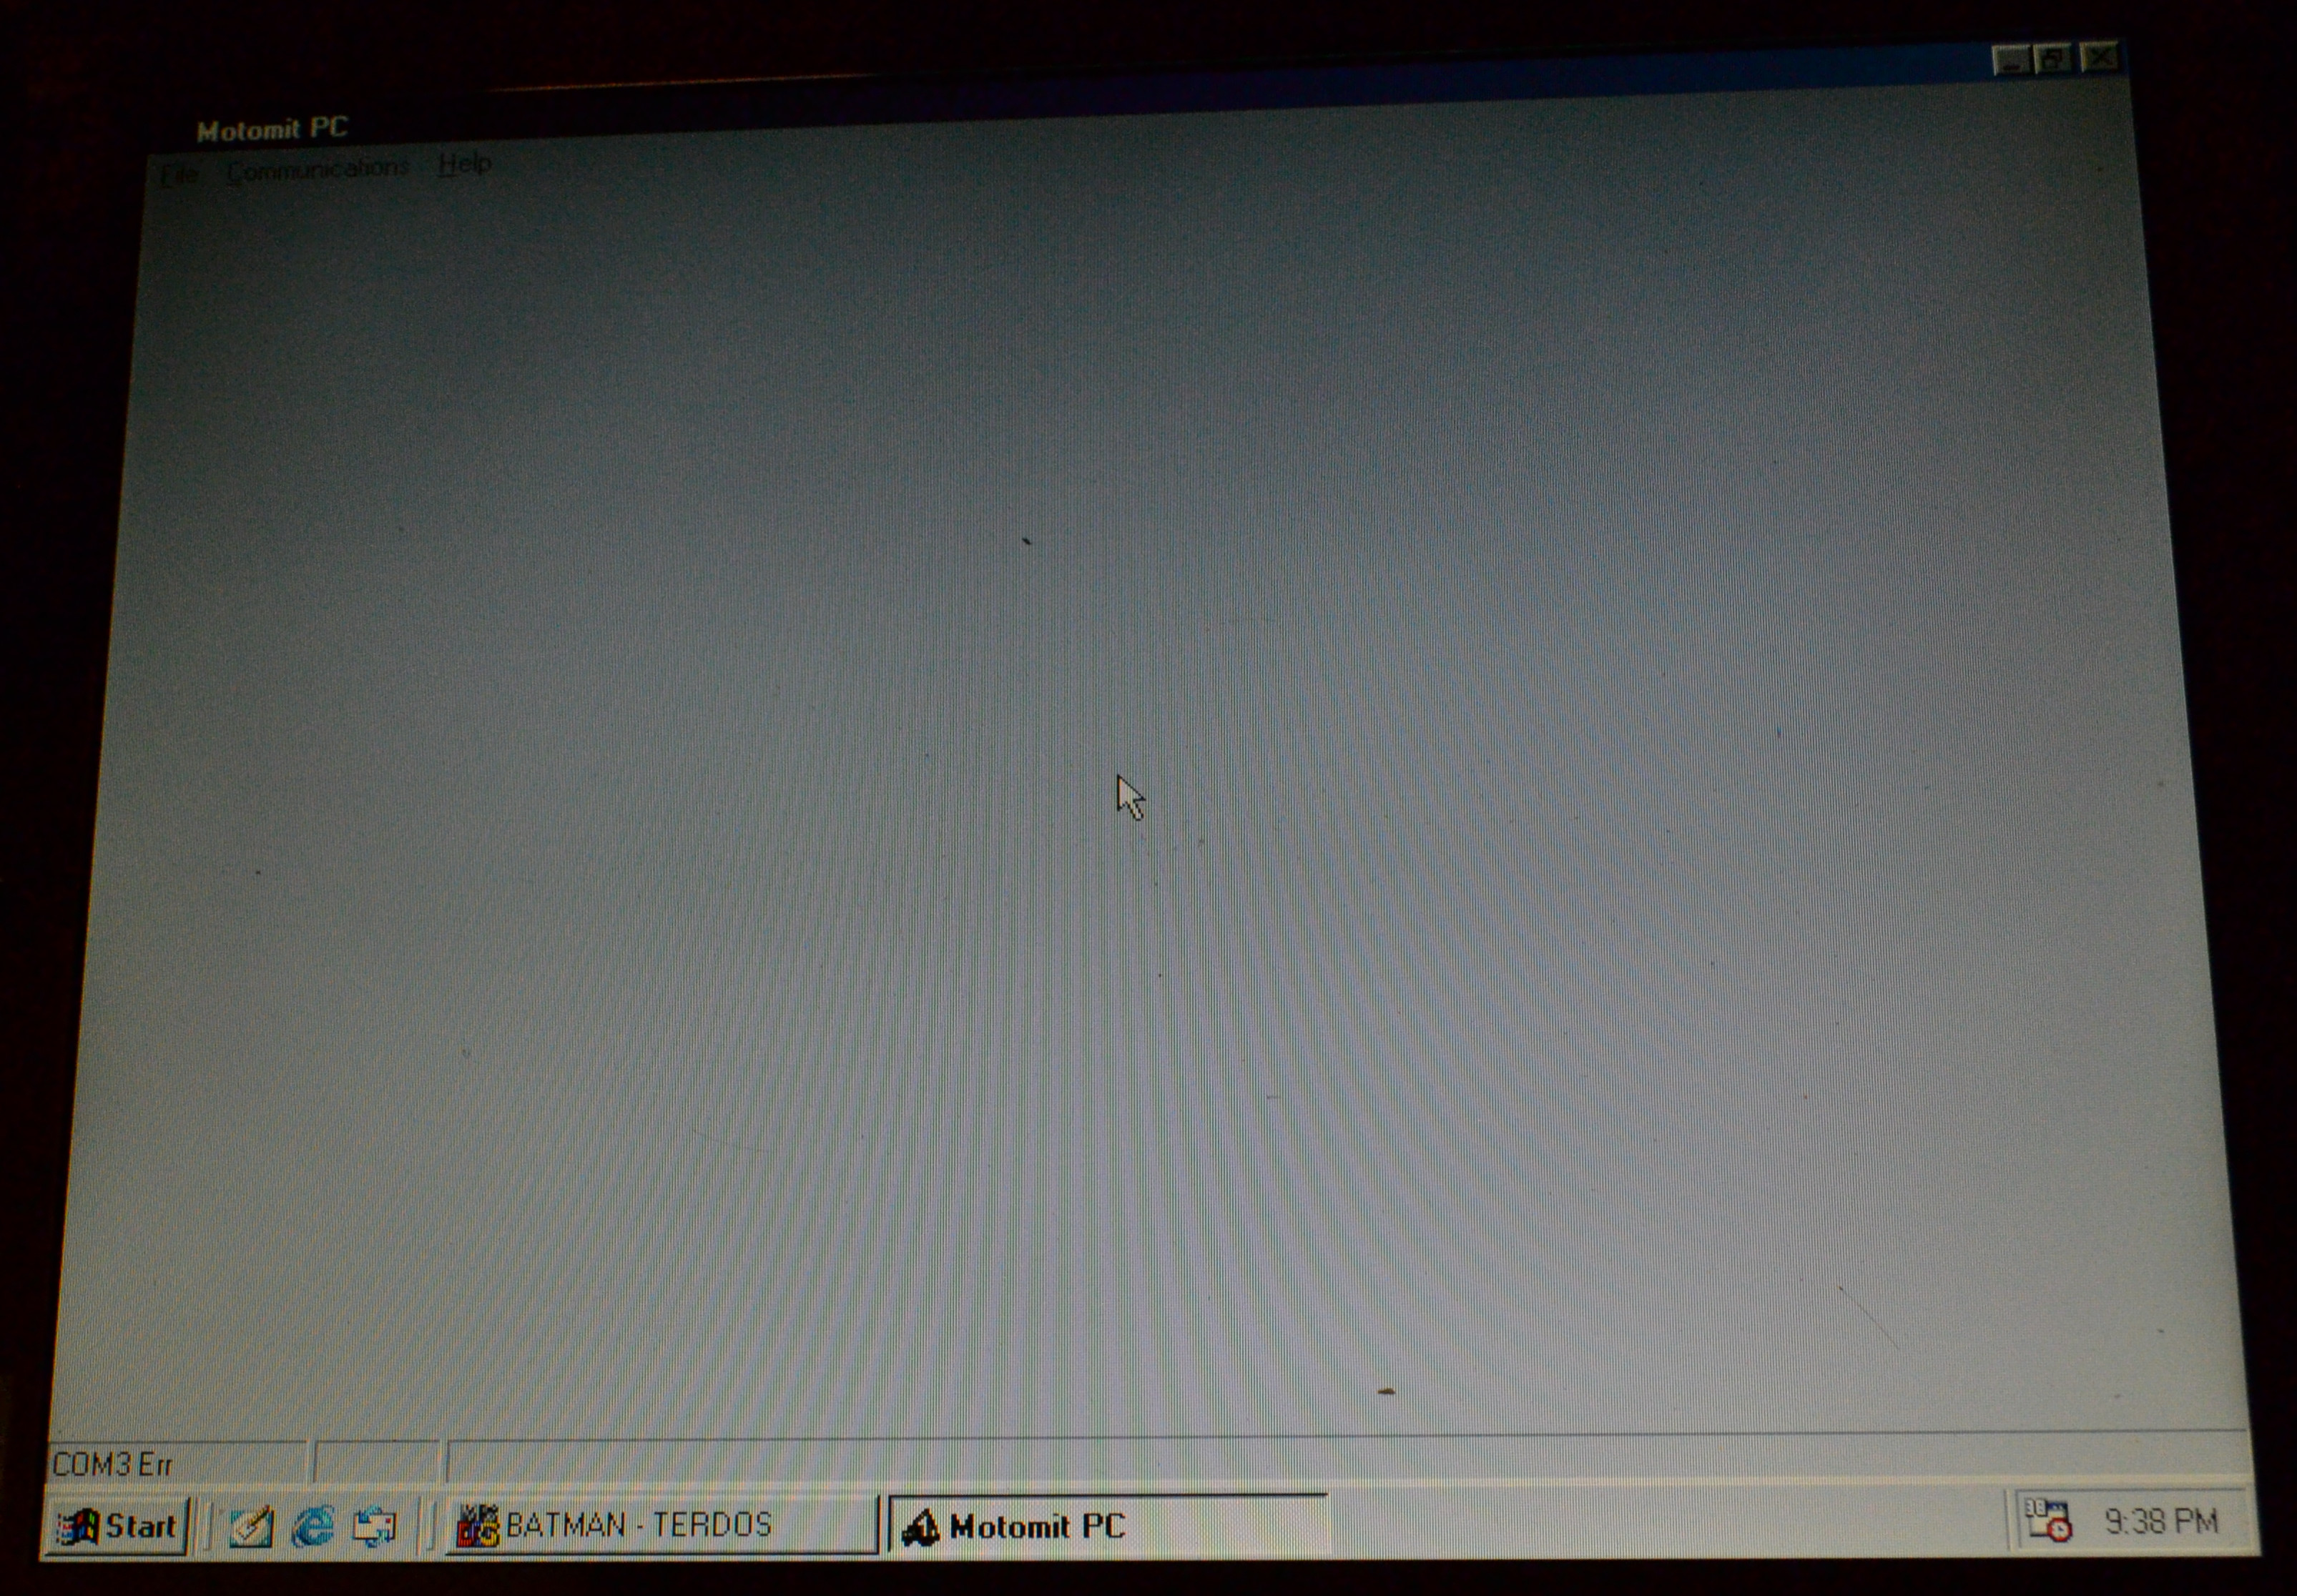
\includegraphics[width=1.00\hsize]{motomit_original.jpg}
\caption{Motomit PC Nero-ajoneuvo-pc:n näytöllä.}
\label{motomit:kuvankaappaus}
\end{figure}

\subsubsection{Ajoneuvo-PC Sunit Nero (Valmet Maxi)}
Hakkuukoneessa käytetty tietokone on kuvassa \ref{kuva_nero} oleva, Sunitin valmistama Sunit Nero (myös nimellä Valmet MAXI) -ajoneuvotietokone. Nero on paketoitu näyttöineen ja keskusyksikköineen yhdeksi all-in-one-tyyppiseksi iskunkestäväksi paketiksi. Vaikka kyseessä ei olekaan sama yksilö, joka on alun perin ollut kiinni hakkuukoneeessa, se on samanlainen kuin alkuperäinen ja samaa ikäluokkaa (noin 17 vuotta, vuodelta 1998). Tietokoneen mitat ovat 315 mm x 252 mm x 115 mm ja paino 4,2 kg. Sunit Neron virrankulutus on noin 25 Wattia.

Nero täyttää CEN:n standardin EN55022 class A- ja class B -vaatimukset, ja Sunit vakuuttaa laitteen täyttävän EU:n direktiivien vaatimukset CE-merkinnällä. Neron kotelointi on tuuletusta lukuun ottamatta IP54-luokkaa, mikä tarkoittaa suojausta pölyltä ja suojausta vesiroiskeita vastaan. \citep{nero:manual}

\begin{figure}[H]
\centering
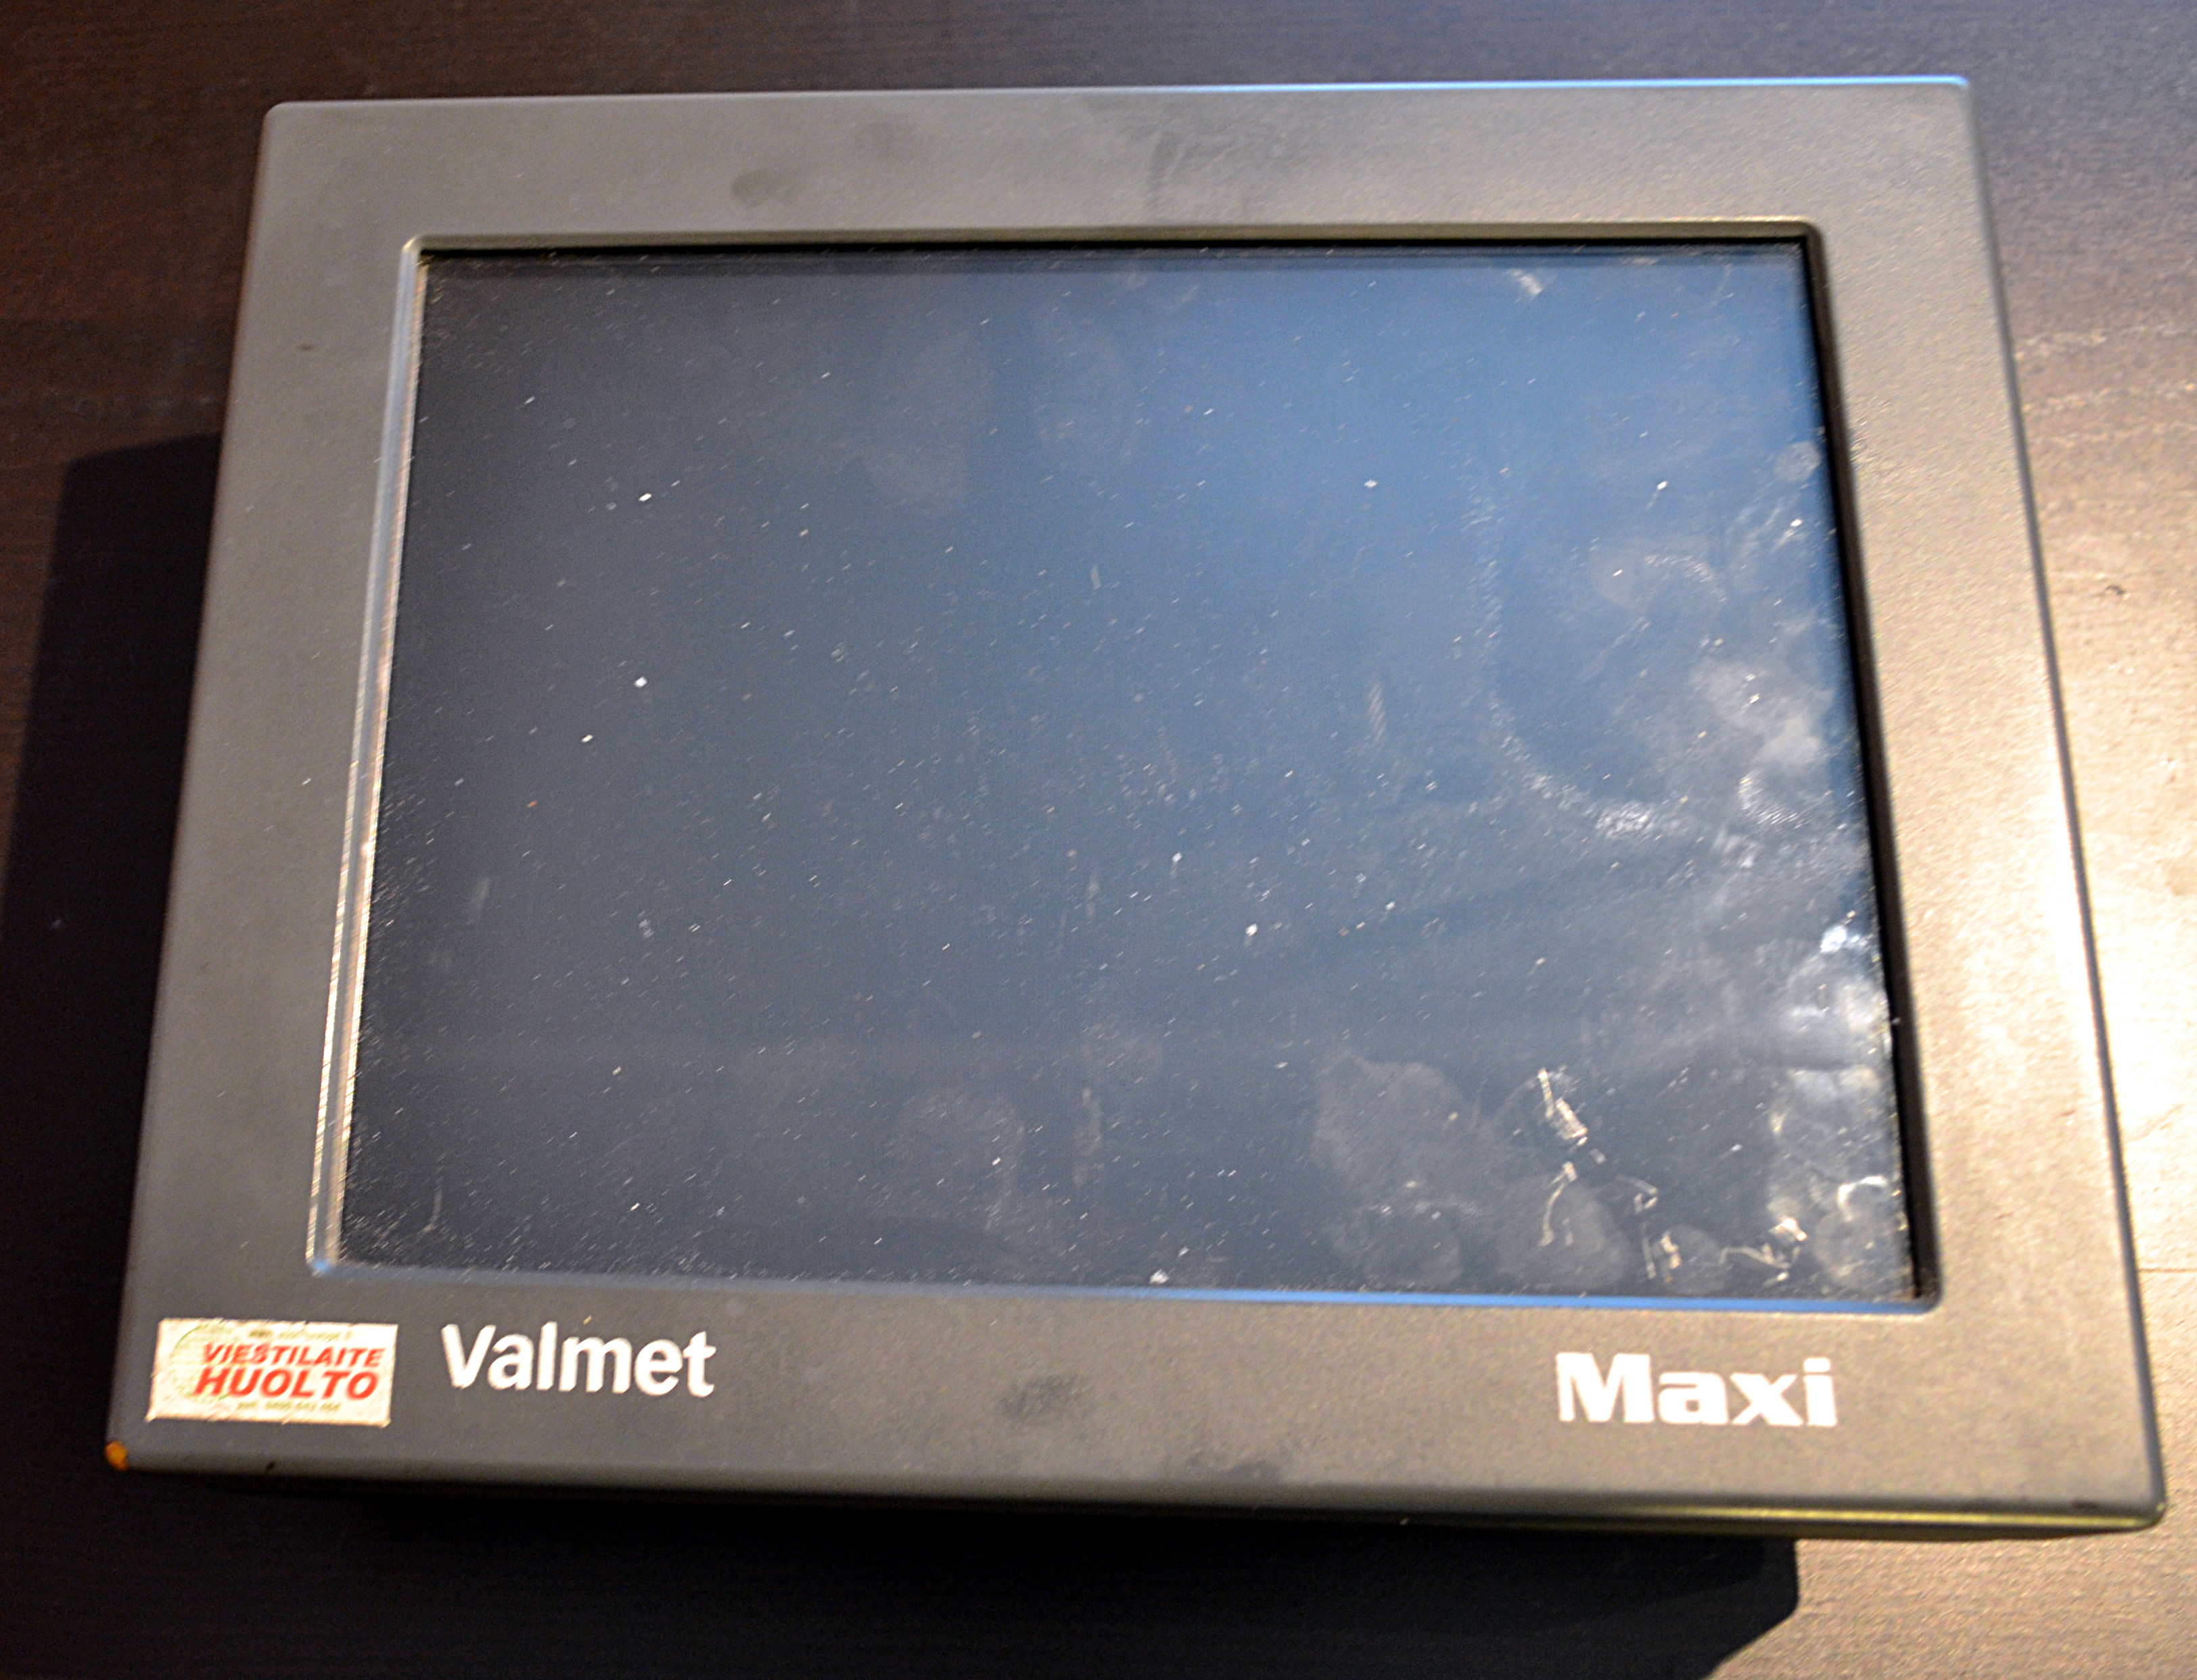
\includegraphics[width=1.000\hsize]{valmet_maxi.jpg}
\caption{Sunit Nero -ajoneuvotietokone.}
\label{kuva_nero}
\end{figure}

Sunit Nero osoittautui olevan toteutettu PC-tekniikalla. Se sisältää tavallisen x86-prosessorin ja Windows 98 -käyttöjärjestelmän. Emolevyn northbridge-ohjaimena on SiS 5571 -ohjain. Tässä Nero-yksilössä prosessorina on AMD:n 300 MHz:n Socket 7 -kantainen K6-prosessori vuodelta 1998 (kuva \ref{kuva_prossu}, alkuperäinen prosessori on vaihdettu useita vuosia sitten tehdyn huollon yhteydessä toiseen) ja 64 Mb keskusmuistia. Tietokoneen kiintolevynä oli tutkintahetkellä Western Digitalin 120 Gb:n Scorpio Blue -kiintolevy, joka sekin on vaihdettu useaan kertaan. Nero-tietokoneessa on 3,5" -levykeasema ja cd-asema. Näyttöpaneeli on 12":n LCD-paneeli 800 x 600 pikselin resoluutiolla. Kuvasuhde on 4:3. Lisäksi koneessa on NiMH-akku BIOSin asetusten säilyttämiseen. Tietokoneessa on liitännät 12 V:n ja 24 V:n jännitteille. \citep{nero:manual}
\newline\newline

\begin{figure}[H]
\centering
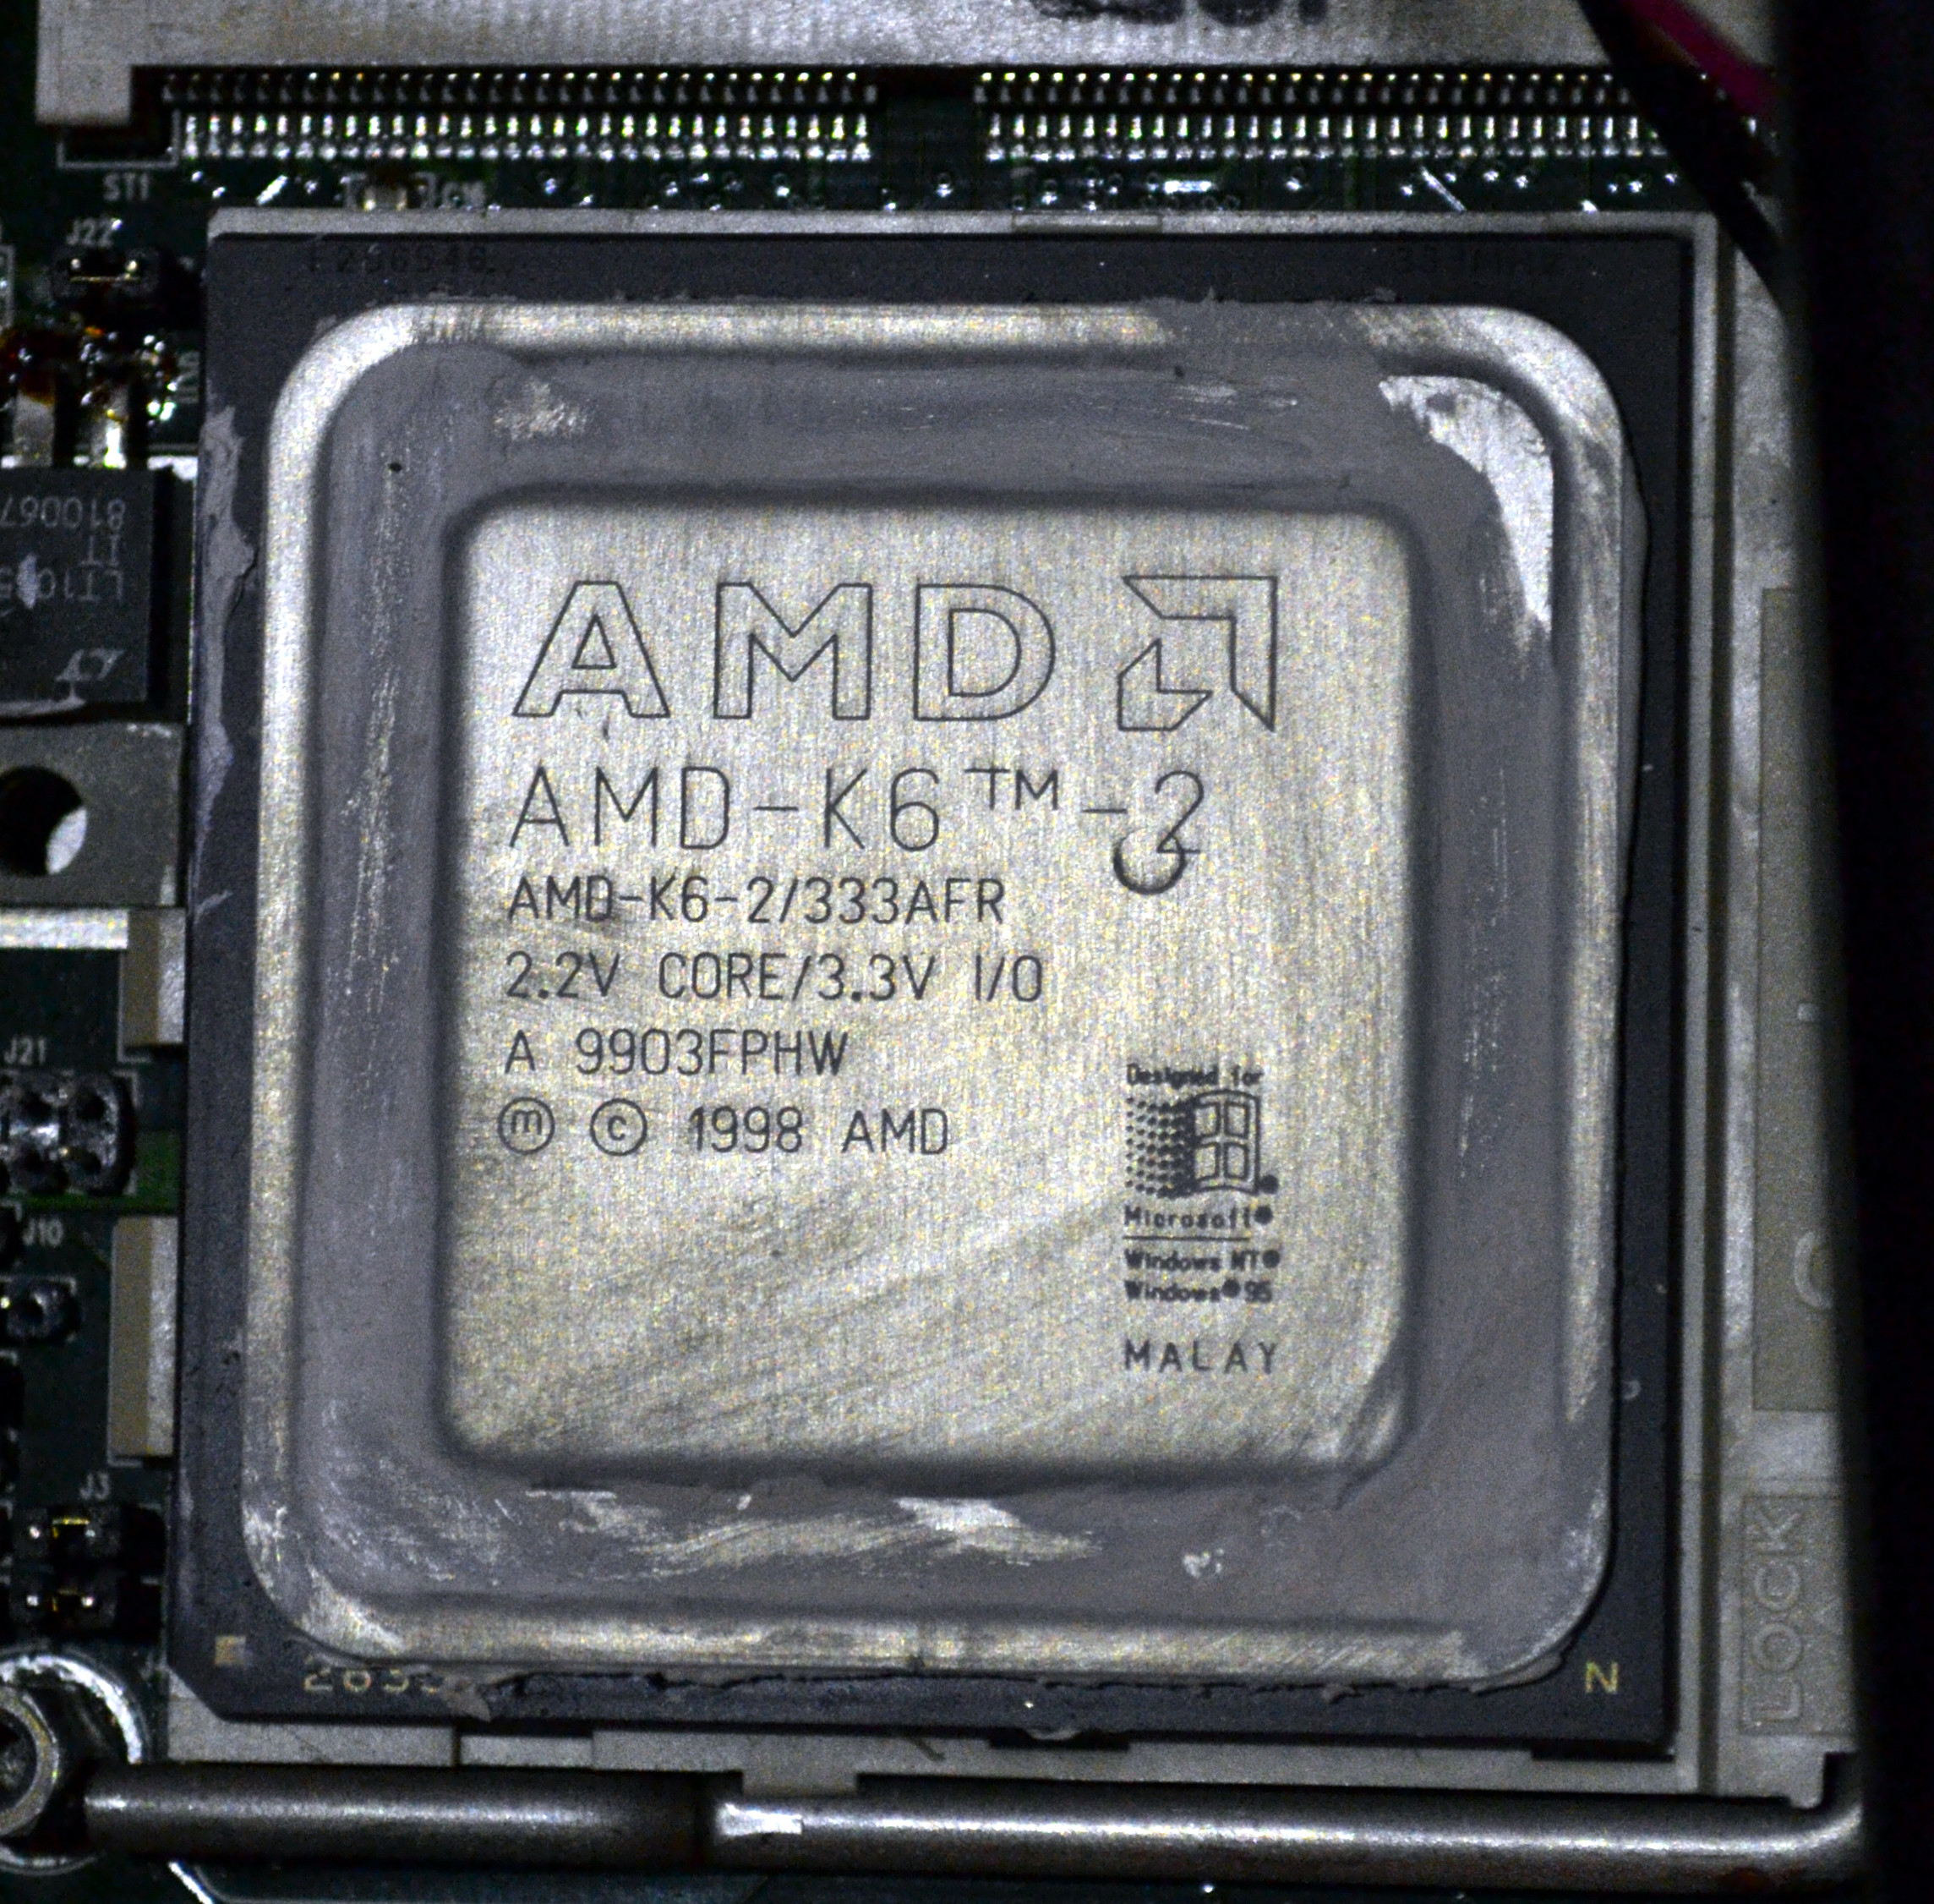
\includegraphics[width=0.800\hsize]{processor.jpg}
\caption{Sunit Neron AMD K6 66 MHz -prosessori}
\label{kuva_prossu}
\end{figure}

Sunitin huolto oli ilmoittanut, ettei se suostu tai pysty enää huoltamaan näin vanhaa tietokonetta, mikä oli myös osasyynä korvaavien vaihtoehtojen kartoittamiseen.

Sunit Nerossa on 3 + 1 sarjaporttiliitäntää (3x 9pin standardi RS-232 -liitintä ja yhdistetty liitin), rinnakkaisporttiliitin (25pin Centronics), Sunitin oma BUS-liitin PS/2-hiirelle ja -näppäimistölle, yhdistetty virta + GPRS + GPS -liitin ja Data I/O-liitin, joka on tarkoitettu optiona oleville CAN- ja SCSI-väylälle, mutta nämä eivät ole kyseisessä yksilössä käytössä (kuva \ref{kuva_liitannat}).  Käytössä on kolme sarjaporttia ja virtaliitin. Sarjaporteista yksi on alkuperäiselle Terman-ohjaukselle, yksi Motomit IT:lle ja kolmas on käytöstä poistetulle GSM-moduulille.

Sunit Neroon on ollut lisäoptiona myös GPS- ja DGPS-moduulit, jotka olisivat mahdollistaneet karttapaikannuksen. Työn kohteena olevassa yksilössä oli GPS-moduuli. Neroon oli liitettynä myös ulkoinen GSM-moduuli \cite{nero:manual}. GPS- ja GSM-moduulit eivät olleet nykyisessä järjestelmässä käytössä, eikä niitä tarvinnut ottaa huomioon korvaavassa tietokoneessa.\newline\newline

\begin{figure}[H]
\centering
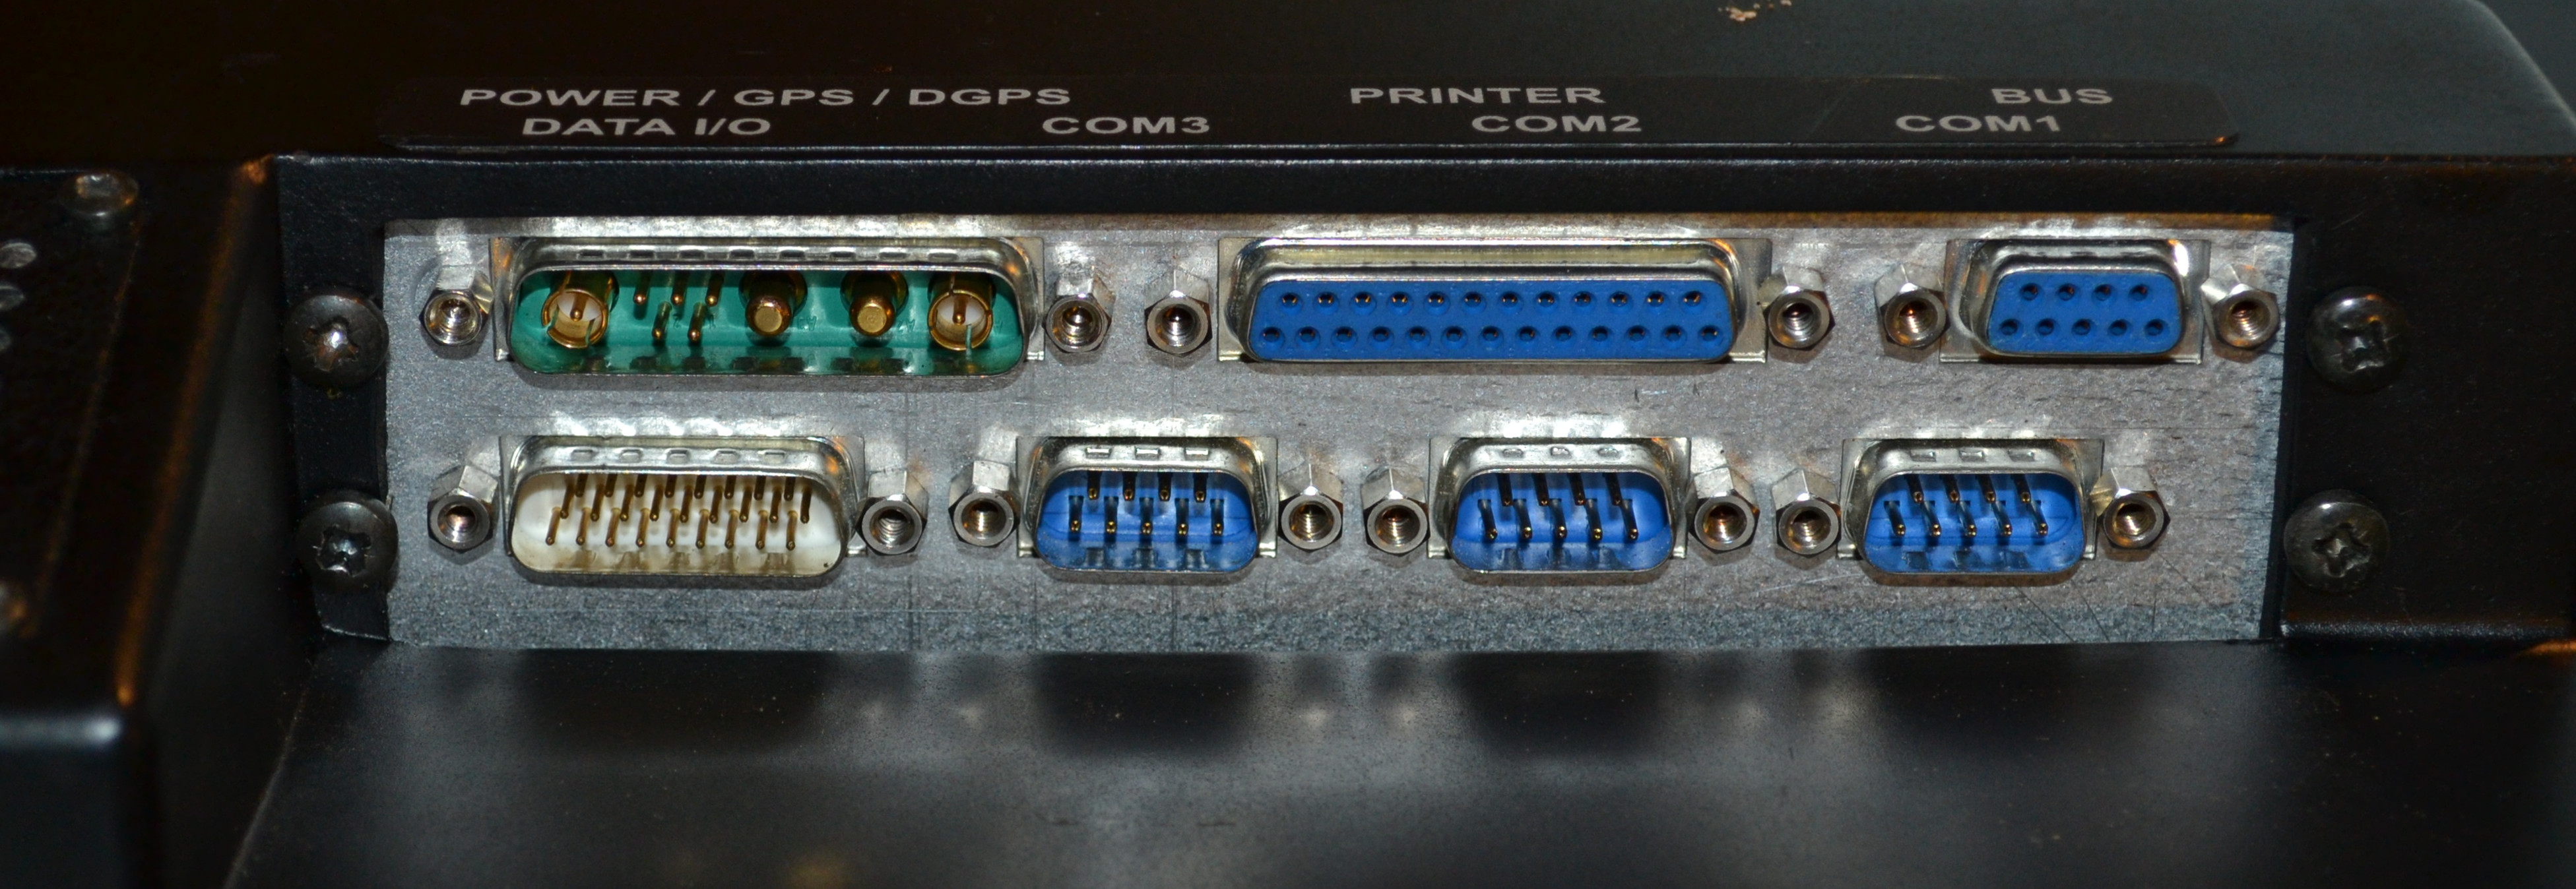
\includegraphics[width=1.00\hsize]{sunit_nero_liitannat.jpg}
\caption{Sunit Neron liitännät.}
\label{kuva_liitannat}
\end{figure}

Sunit Nero on rakennettu kolmeen kerrokseen kahden 31 cm x 23 cm -kokoisen metallilevyn väliin, jotka on ankkuroitu koteloon kiinni neljällä  läpivientiruuvilla. Ensimmäisessä kerroksessa on Neron käyttämä emolevy, keskellä kiintolevy, levykeasema, cd-asema ja vara-akku. Viimeisessä kerroksessa on 12":n LCD-näyttöpaneeli.

\subsubsection{Valmet Terman -ohjelmisto}
Terman on Valmetin alkuperäinen DOS-pohjainen hallinta- ja apteerausohjelmisto käytettävälle hakkuukoneelle (kuva \ref{kuva_terman}). Ohjelmiston versio on riippuvainen käytettävästä hakkuukoneesta. Hakkukoneen kanssa kommunikoidaan 9600 bitin nopeudella RS-232-sarjaporttia käyttäen. Koska mittauslaite on vaihdettu Motomit IT-järjestelmälle, käytetään Termania lähinnä hakkuukoneen ajo- ja moottoriasetusten hallintaan.
\newline\newline

\begin{figure}[H]
\centering
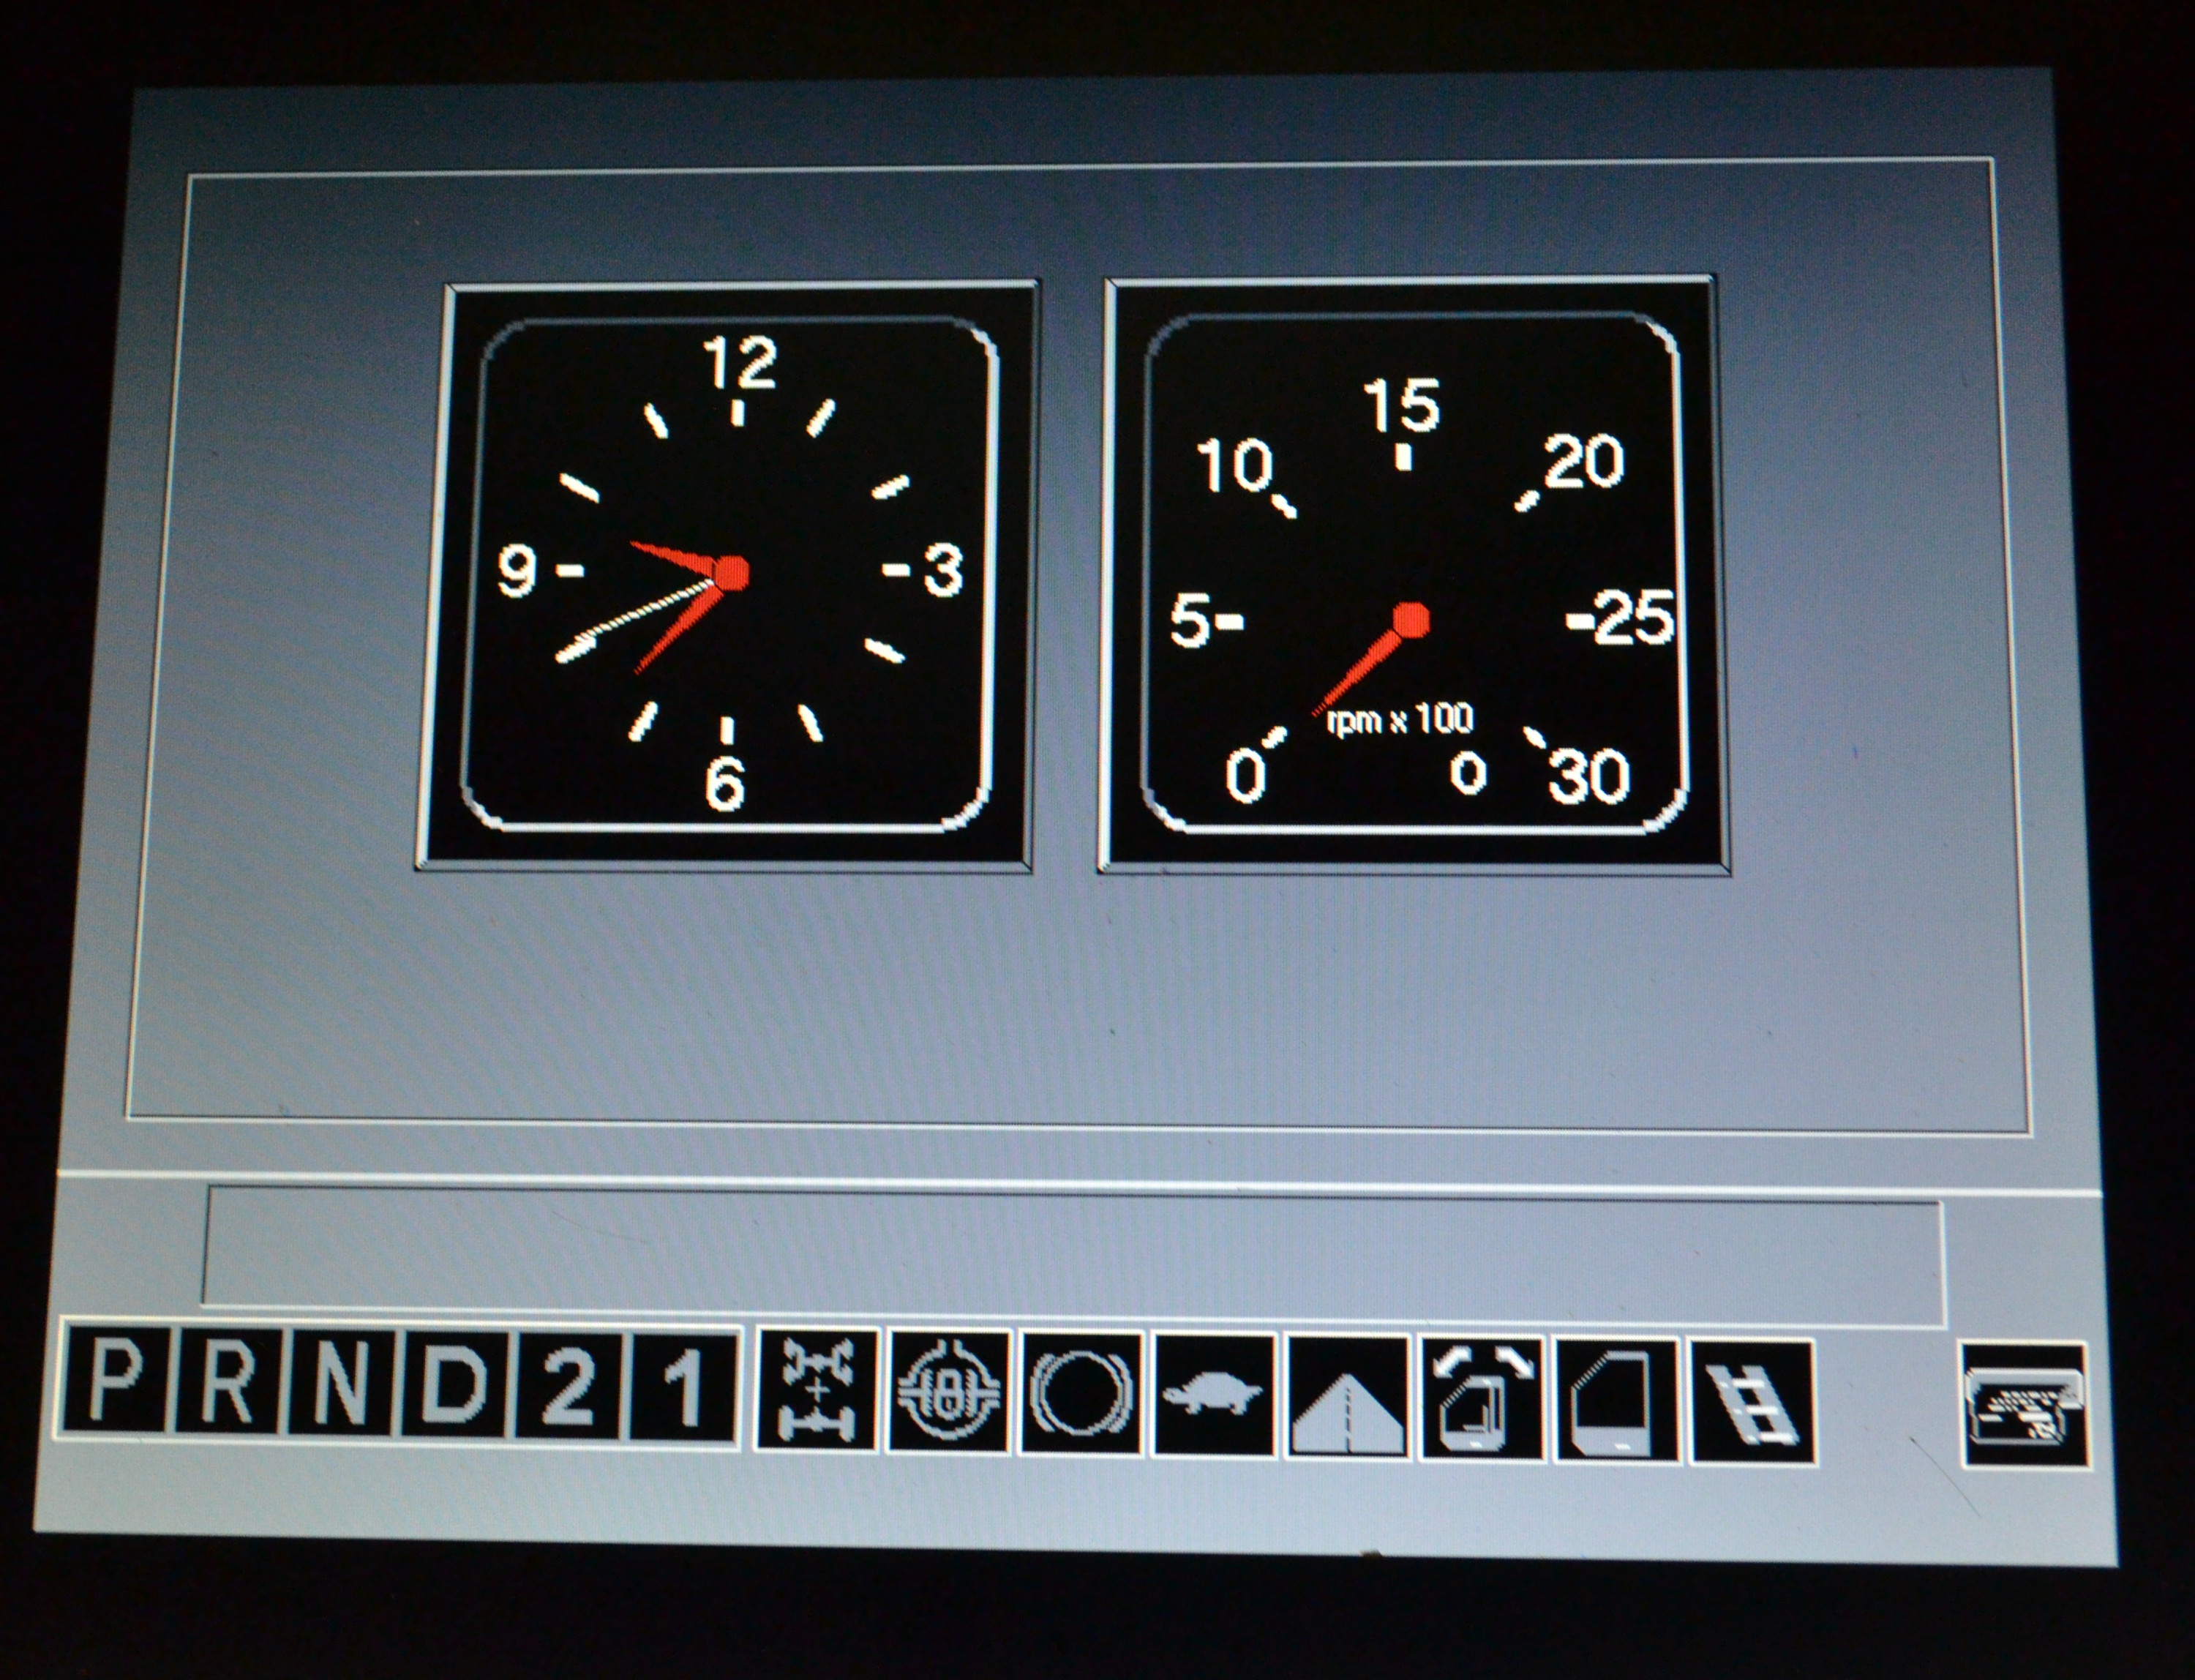
\includegraphics[width=1.00\hsize]{terman_original.jpg}
\caption{Terman-ohjelma Nero-ajoneuvo-pc:n näytöllä.}
\label{kuva_terman}
\end{figure}

%\newpage
\subsubsection{Päälohkokaavio}
Kuvan \ref{kuva_lohkokaavio} lohkokaavioon on kuvattu Valmet 901 -hakkuukoneen tärkeimmät osat, niiden käyttämät väylät ja alkuperäisessä järjestelmässä olleet laitteet. Hakkuukoneessa ei ole itsessään käytössä vielä CAN-väylää, mutta jälkikäteen asennettu hakkuupää ja Motomitin mittalaitejärjestelmä käyttävät CAN-väylää sisäisesti ja hakkuupään ohjaukseen. Hakkuukoneen alkuperäiset järjestelmät on ohjattu jokainen laite omalla ohjausjohtimellaan. Kaaviosta näkyvistä järjestelmistä korvattiin keltaisella näkyvä Nero-ajoneuvotietokone ja siihen liitetyt hiiri ja näppäimistö.

\begin{figure}[H]
\centering
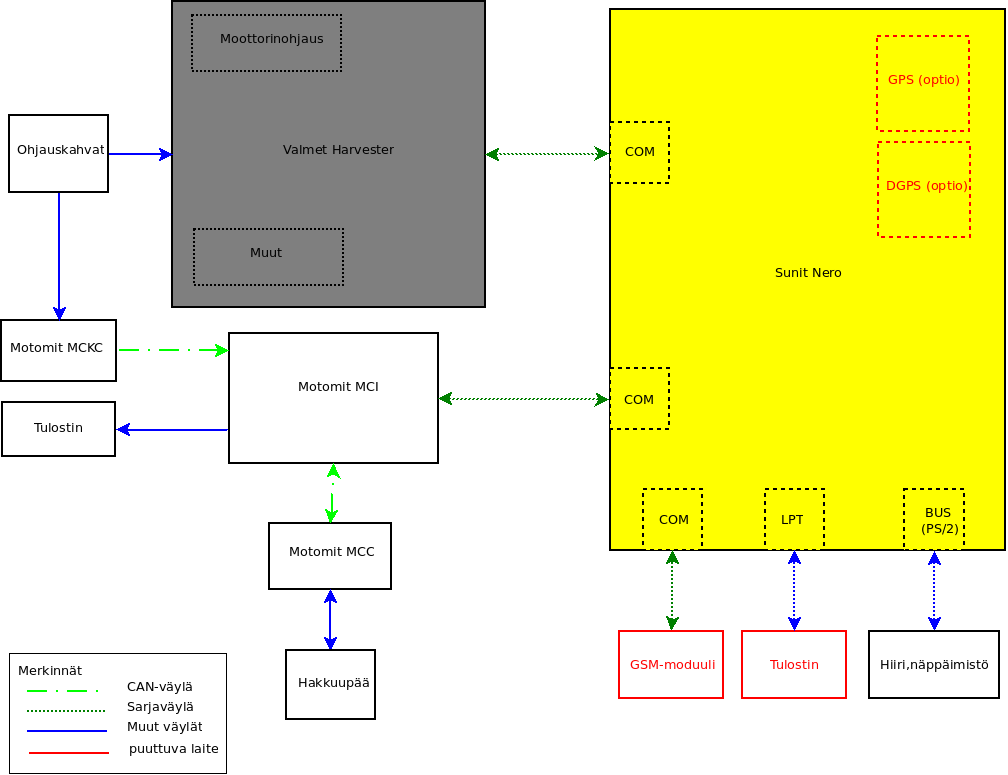
\includegraphics[width=1.00\hsize]{saatanan_kaavio.png}
\caption{Hakkuukoneen järjestelmien lohkokaavio.}
\label{kuva_lohkokaavio}
\end{figure}

\newpage
\chapter{Ohjelmistojen siirron mahdolliset toteuttamisvaihtoehdot}

Loppukäyttäjän (hakkuukoneen kuljettajan) toiveena oli, että tietokoneen vaihtuessa käytössä olevat Terman- ja Motomit PC -ohjelmistot toimivat uudessa koneessa samaan tapaan kuin vanhassa ja näkyvät samalla tavalla kuin ohjelmistot aiemminkin ovat näkyneet. Loppukäyttäjän toiveiden lisäksi oli huomioitava tietokoneen käyttöolosuhteiden asettamat vaatimukset ja aiheeseen liittyvä lainsäädäntö ja standardit.

\section{Natiivi ympäristö}
Natiivilla ympäristöllä tarkoitetaan, että laitteiston ja käyttöjärjestelmän välissä ei ole virtualisointi- tai yhteensopivuusrajapintaa, vaan käyttöjärjestelmällä on suora pääsy fyysisen laitteiston rajapintoihin.

% Natiivin ympäristön hyviä puolia:
% * Suoritusnopeus
% * Ohjelman ja laitteiston välisen kommunikoinnin kutsupolku? lyhyempi
% * toimiessaan yksinkertaisin

% Natiivin ympäristön Haittapuolia ja rajoituksia:
% * Vanhat käyttöjärjestelmät eivät toimi uusien laitteiden kanssa
% ** koska ei löydy laiteajureita
% ** koska uudet laitteet ovat liian nopeita tai liian isolla kapasiteetilla varustettuja suhteessa vanhojen käyttöjärjestelmien toteutuksiin
% * Uudet käyttöjärjestelmät eivät ole välttämättä yhteensopivia vanhojen ohjelmien kanssa
% * (ei liity työhön)
% ** Hyötysuhde huono
% ** Kaikilla ohjelmilla (käyttöjärjestelmästä riippuen) pääsy toisensa tiedostoihin


Natiivin ympäristön vaihtoehdossa ohjelmistoja käytetään ympäristössä, johon ne on aikoinaan suunniteltu toimivaksi. Hyvänä puolena tässä vaihtoehdossa on, että ohjelmat toimivat varmasti siten, kuin ne on suunniteltu. Koska käytettävät ohjelmistot ovat vanhoja, DOS- ja Windows 98 -aikaisia, vaatisi natiivin ympäristön käyttäminen kuitenkin alkuperäisen tietokoneen kanssa suunnilleen samaa ikäluokkaa olevan laitteiston käyttämisen. Uudemmat laitteistot eivät ole enää yhteensopivia Windows 98SE / ME:n kanssa, ja lisäksi Windows 98:lla on maksimirajoituksia käytettävälle laitteistolle kuten luotettavasti toimiva määrä keskusmuistia on maksimissaan 1024 Mb ja kiintolevyosiolle rajattu maksimikoko on 127,5 Gb \cite{win98:maxspecs}. Uudemmille laitteille ei myöskään löydy välttämättä toimivia ajureita, mikä rajoittaa entisestään mahdollisia laitteistovaihtoehtoja. Koska ajoneuvotietokone ei ole yhdistettynä Internetiin ja koneelle on rajattu pääsy, ei tässä käyttöympäristössä Windows 98:n paikkaamattomilla haavoittuvuuksilla (Windows 98: 84 kpl, Windows 98SE 61 kpl \cite{win98:vulns}) ole erityistä merkitystä käytettävyyteen.

\section{Ohjelmistojen rajapintojen yhteensopivuuskerros}
Käyttöjärjestelmän ja ohjelmiston välissä voidaan suorittaa erillistä rajapintasovellusta, joka toteuttaa toisen käyttöjärjestelmän järjestelmäkirjastot ja järjestelmäkutsut ja mahdollistaa näin muuten yhteensopimattomien, mutta samaa prosessoriarkkitehtuuria käyttävien ohjelmistojen suorituksen \cite{ntvdm_kb}. Ohjelmistojen rajapintojen yhteensopivuuskerrosvaihtoehdossa käytetään käyttöjärjestelmän ja ohjelman välissä sopivia rajapintakerroksia, jolloin saadaan käyttöjärjestelmän kanssa yhteensopimattomat ohjelmat toimimaan keskenään. Vaihtoehto vaatii yhteensopivan laitteistoarkkitehtuurin alkuperäisen järjestelmän kanssa (x86). Nykyiset Windows-versiot (Windows XP+) sisältävät jo valmiiksi yhteensopivuustilan, joka mahdollistaa vanhempien ohjelmien käyttämisen uudemmissa käyttöjärjestelmissä. Linuxissa Wine-rajapinta mahdollistaa kaikenikäisten Windows-sovellusten suorittamisen Linuxissa. Myös DOS:lle on olemassa rajapintakerrostoteutus Linuxiin.

\subsubsection{NTVDM ja WOW}
Virtual Dos Machine mahdollistaa DOS-ohjelmien suorituksen muissa käyttöjärjestelmissä. VDM-toteutuksia on ollut olemassa Windowseista 3.x-käyttöjärjestelmästä lähtien, ja OS/2 sisälsi hyvän DOS-tuen oman MVDM-toteutuksensa takia. VDM on toteutettu myös Wineen lähinnä 16-bittisten Windows 3.x -ohjelmien tuen takia. 16-bittisten ohjelmien tukea tarvitaan työssä Terman-ohjelmistolle.

NTVDM (NT Virtual DOS Machine) ja WOW (Windows On Windows) ovat Windows-käyttöjärjestelmän alijärjestelmiä, jotka mahdollistavat DOS- ja 16-bittisten Windows 3.x-ohjelmien suorittamisen uudemmissa NT-ytimeen pohjautuvissa Windows-versioissa. NTVDM oli toteutettu emulaattorina myös Windows NT:n MIPS- ja Alpha-versiolle. NTVDM ja WOW on poistettu 64-bittisisistä Windows-versioista. \citep{ntvdm_2}

NTVDM emuloi x86-prosessorin suorittamaa MS-DOS-käyttöjärjestelmää. Se tulkkaa DOS-ohjelmien tekemät suorat laitteiston manipulointipyynnöt Windowsin API-pyynnöiksi. Emuloitujen laitteistojen tuki on kuitenkin NTVDM:ssä yksinkertainen ja rajoittunut. Se ei rajaa ohjelmien suoritusnopeutta, jolloin moni DOS-ohjelma suoritetaan nykylaitteistolla liian nopeasti, eikä kommunikointi laitteiston kanssa välttämättä onnistu, koska ohjelmat eivät odota vastausta tarpeeksi pitkään. Työn kannalta nämä NTVDM:n rajoitukset tulevat esteeksi, jotta Terman-ohjelmiston saisi kommunikoimaan sarjaväylälaitteen kanssa luotettavasti.

NTVDM:n ratkaisu DOS:n tietoturvaongelmiin on suorittaa jokaista DOS-ohjelmaa omassa VDM-prosessissaan, jolloin ohjelmat ovat suojattuja toisiltaan. DOS-ohjelmien kaatuminen ei vaikuta muihin suoritettaviin prosesseihin, koska jokainen suoritettava DOS-ohjelma on oma VDM-prosessinsa. Uudemmissa käyttöjärjestelmissä (Windows 7+) voi määritellä, suoritetaanko DOS-ohjelmat omina prosesseinaan vai yhden VDM-prosessin alla.

WOW (Win16 on Win32) on Windowsin alijärjestelmä, joka täydentää NTVDM:ään tuen 16-bittisille Windows-ohjelmille. Win16-ohjelmat suoritetaan yhdessä VDM-prosessissa omina säikeinään. Tällä tavoin on saatu aikaan paras yhteensopivuus Windows 3.x:n kanssa. Haittapuolena tulee jaettu muistiavaruus kaikkien 16-bittisten ohjelmien kanssa, ja se voi aiheuttaa epävakautta alijärjestelmän sisällä. Alijärjestelmän kaatuminen sulkee kaikki 16-bittiset ohjelmat, mutta ei vaikuta käyttöjärjestelmän toimintaan muuten. \citep{ntvdm_kb}


\subsubsection{Wine-yhteensopivuuskerros}
%https://www.winehq.org/docs/winedev-guide/x2884
Wine on POSIX-yhteensopiville käyttöjärjestelmille kehitetty yhteensopivuuskerros, jolla 32- ja 64-bittiset Windows-ohjelmat saadaan toimimaan muissa käyttöjärjestelmissä. Wineen on toteutettu Windowsin ytimen järjestelmäkutsut ja useita tarvittavia DLL-kirjastoja. Työssä tarvitaan 32-bittistä Windows-tukea Motomitin hallintaohjelmistolle. Motomitin toimivuus testattiin Winen kanssa. Vanhempia versioita Motomitistä ei saatu toimimaan, mutta uudemmat Windows 7 -yhteensopivat versiot Motomitistä ovat myös Winen kanssa yhteensopivia.

Winen 1.0-versio julkaistiin vuonna 2008. Uusi vakaa versio kahden vuoden välein. Viimeisin vakaa versio on 1.6. Wine käyttää versionumeroinnissaan sekventiaalista Major.Minor.Build-tyyliä, jossa parilliset Minor-versiot ovat vakaita julkaisuita ja parittomat kehitysversioita.

Wineen pystyy asettamaan käyttöön tarvittaessa alkuperäisen järjestelmän jaettuja DLL-kirjastoja. Alkuperäinen DLL tarjoaa täyden yhteensopivuuden kirjaston toteuttamille rutiineille. Näiden käytön vaarana on, että ne voivat yrittää käyttää Winestä puuttuvia Windowsin järjestelmäkomponentteja, jolloin ohjelman toiminnallisuus kärsii. Winen sisäänrakennetut DLL:t sisältävät tarvittavilta osin lisäyksiä ja käärekoodia, joilla kirjastot saadaan toimimaan yhteem Unixissa käytettyjen ratkaisujen kanssa.

Winen ytimen (kuva \ref{wine_pino}) ratkaisut eivät sisällä mahdollisuutta Windowsin ajurien käyttöön. Tiettyjä laitteita tuetaan, mikäli niille löytyy käytettävästä käyttöjärjestelmästä ajurituki ja jos itse Wineen on toteutettu tarvittavat rajapintamuunnokset. Winessä on kuitenkin ohitettu ajurien tarve toteuttamalla monet DLL-kirjastot siten, että ne käyttävät suoraan Unixin rajapintoja (tulostus, äänet, näyttö). Jokainen Wine-prosessi (suoritettava Windows-ohjelma) suoritetaan omana prosessina, jolloin niillä on omat osoiteavaruudet, eikä niillä ole pääsyä muiden Winen suorittamien ohjelmien muistialueille.

Winen kehitys alkoi jo vuonna 1993, kun sen alkuperäinen kehittäjä Bob Amstadt halusi suorittaa senaikaisia Windows 3.1 -ohjelmia Windowsin puolella. Kehitysvastuu siirtyi vuonna 1994 Alexandre Julliardille, joka on toiminut Wine Projectin johtohahmona ja projektin vetäjänä siitä lähtien. Vapaaehtoiset kehittäjät ovat kirjoittaneet noin puolet Winen koodista. Yrityspuolelta projektin pääasiallinen sponsori on CodeWeavers, jonka työntekijöitä myös moni Wine-kehittäjä on. CodeWeavers on kehittänyt CrossOver Linux-tuotteensa joka on kaupallistettu, käyttäjäystävällisempi versio Winestä. CodeWeavers tarjoaa myös ohjelmistojen porttaus- ja tukipalveluita Winelle. \citep{wine:codeweavers}


\begin{figure}[H]
\centering
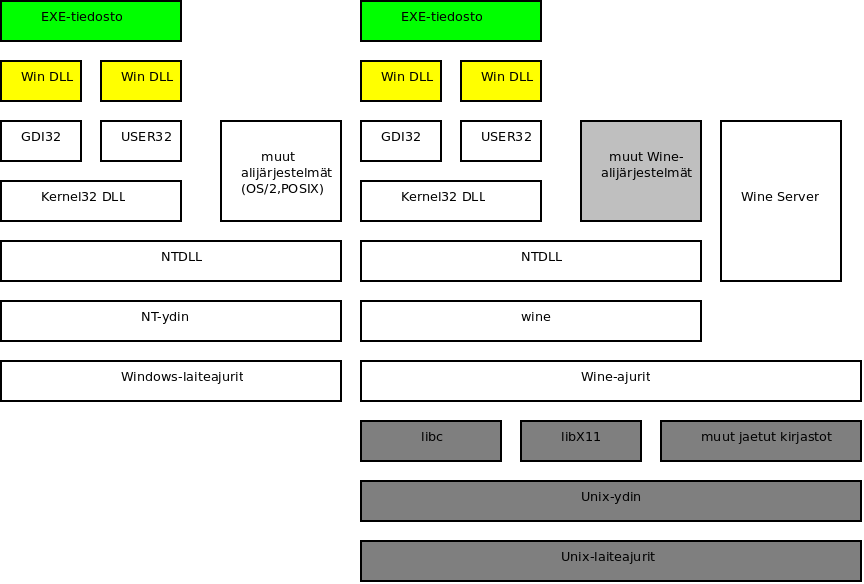
\includegraphics[width=1.00\hsize]{kaaviot/wine_pino.png}
\caption{Vasemmalla Windows NT:n käyttämä arkkitehtuuri, oikealla Wineen toteutettu arkkitehtuuri \cite{wine:winnt_architecture,wine:architecture}. }
\label{wine_pino}
\end{figure}

Wine-palvelimen avulla on totetutettu IPC:n (prosessien välinen kommmunikointi) synkronointi ja prosessien hallinta. Windows-alijärjestelmistä on toteutettuna vain Win32-alijärjestelmä (Kernel32). Winen toteuttamien DLL-tiedostojen nimeämiskäytäntö on pyritty pitämään mahdollisimman lähellä Windowsin nimeämiskäytäntöä, jos vain se on ollut mahdollista. \citep{wine:architecture}

\subsubsection{Dosemu}
% Mikä doesmu
%mitä tulkitaan
% mitä emuloidaan
Dosemu on Linuxille kehitetty yhteensopivuuskerros, jolla saa suoritettua 16-bittisiä DOS-ohjelmia x86/x64-arkkitehtuuria käyttävässä Linux-käyttöjärjestelmässä. Dosemu on käyttäjätason ohjelma (ei vaadi pääkäyttäjän oikeuksia), joka hyödyntää 80386:n ja Linux-ytimen erityisominaisuuksia suorittaakseen DOS-ohjelmia eriytettynä prosesseina. Dosemu virtualisoi kaiken I/O-liikenteen, emuloi laitteet, joihin DOS-ohjelmilla on suora pääsy ja tarjoaa virtuaalisen kiintolevyn, joka oikeasti on tiedostopolku Linuxissa. Dosemu on yhtenä mahdollisuutena Terman-ohjelmiston suorittamiseen kohdejärjestelmässä.

Tekstipohjaiset DOS-ohjelmat saa suoritettua Dosemun avulla suoraan konsolissa, mutta siinä on lisäksi CGA/EGA/VGA-emulaatio DOS:n graafista moodia käyttäville ohjelmille (DOS:n Mode 13h eli resoluutio 320 x 200 ja 256 väriä). Dosemu sisältää myös tuen sarja- ja rinnakkaisporteille.

% http://www.dosemu.org/docs/HOWTO/x596.html#AEN598
Dosemun kehitys alkoi vuonna 1992 Matthias Lautnerin toimesta. Projektin vastuuhenkilö on vaihtunut vuosien varrella, ja vuodesta 2004 lähtien vastuussa on ollut Bart Oldeman. \citep{dosemu:history}

%Tähän vitun hieno kaavio? DOS on kyllä niin aneeminen että en tiedä löytyykö



\section{Virtualisointi}
Virtualisoinnissa alkuperäisiä ohjelmistoja ja käyttöjärjestelmää suoritetaan virtuaalikoneessa toisen käyttöjärjestelmän päällä. Näin saavutetaan varmin yhteensopivuus ohjelmistotasolla. Oheislaitteiden siirtämisessä virtualisoidun koneen käyttöön on rajoituksia, jotka pitää huomioida virtualisointiohjelmistoja valittaessa. Vaihtoehto kuluttaa muistia enemmän ja on hieman hitaampi kuin natiivi toteutus. Hyötysuhde on noin 90 \%  natiivista. \citep{virtnat_anadtech}

%KORJAUSKOMMENTTI: Viittaa lähteeseen!
% KKOMMENTTI: Lähdeviittaukset olemassa, ei docx:ssä

Koska virtualisointi on varsin yleistä, virtualisointiratkaisuja tarjoavia yrityksiä ja ohjelmistoja on paljon. Työpöytävirtualisointiin riittävillä ominaisuuksilla (mm. sarjaporttien välitys virtuaalikoneille) sopii esimerkiksi avoimen lähdekoodin QEMU-hypervisori tai Oraclen Virtualbox-hypervisori. Myös Microsoft tarjoaa Windows-ympäristöön VirtualPC-hypervisoria. Kaupallisista tarjoajista VMWarella on olemassa VMWare Workstation- ja VMWare Player -hypervisori. Virtualisoinnin avulla pyritään suorittamaan alkuperäisen ajoneuvotietokoneen Windows 98 -käyttöjärjestelmää ja ohjelmia ilman erillisiä rajapintakerroksia.

Hypervisorit on jaettu kahteen tyyppiin: 1-tyypin natiiveihin hypervisoreihin, joita suoritetaan laitteiston ja käyttöjärjestelmän välissä, ja 2-tyypin ''hosted''-hypervisoreihin, jotka suoritetaan tavallisina ohjelmina käyttöjärjestelmästä. Jako ei kuitenkaan ole kaikkien hypervisoreiden kohdalla näin selvä. %(wink wink KVM)


\subsubsection{Virtuaalikoneet}
\subsubsection{Xen}
%http://wiki.xenproject.org/wiki/Xen_Overview
%QEMU is involved only in the emulation of hardware; the execution of the guest is done within Xen and is totally hidden from QEMU.
Xen on Cambridgen yliopistossa kehitetty 1-tyypin hypervisor. % http://www.xenproject.org/about/history.html
Xenin kehitystyö aloitettiin 1990-luvun loppupuolella Xenoserver-projektin yhteydessä, ja ensimmäinen julkinen avoin versio julkaistiin lokakuussa 2003, minkä jälkeen uusia versioita on julkaistu säännöllisesti; uusin on versio 4.5 \cite{xen_history}. Xen suoritetaan käynnistyslataimesta (bootloaderista), jolloin se asettautuu laitteiston ja virtuaalikoneiden väliin kuvassa \ref{kuva_xen} olevan arkkitehtuurikavion mukaisesti. Xen vaatiikiin aina suoritettavaksi yhden virtuaalikoneen eli niin sanottu isäntäkoneen eli Dom0:n. Dom0 hoitaa interaktion laitteiston ja muiden virtuaalikoneiden kanssa. Lisäksi ainoastaan Dom0:lla on pääsy Xenin rajapintaan, minkä kautta hallitaan järjestelmää.

Xen vaatii erillisen tuen kohdekäyttöjärjestelmiltä, jotta niitä voidaan käyttää Xenin avulla paravirtualisoituina (poikkeuksena laitteistoavustettu virtualisointi, jolloin kohde ei tarvitse muutoksia). Tuki Xenin paravirtualisoinnille on kuitenkin useimmissa Linux- ja BSD-jakeluissa. Windowsissa ei ole tukea Xenin paravirtualisoinnille, mutta sitä voidaan suorittaa laitteistoavusteisen virtualisoinnin avulla Xenin päällä. Xen on tarkoitettu palvelinten virtualisointiin, ja siten sen ratkaisut ja toteutus tekevät siitä epäkäytännöllisen tätä projektia ajatellen. \citep{xen_overview}

%The Control Domain (or Domain 0) is a specialized Virtual Machine that has special privileges like the capability to access the hardware directly, handles all access to the system’s I/O functions and interacts with the other Virtual Machines. It also exposes a control interface to the outside world, through which the system is controlled. The Xen Project hypervisor is not usable without Domain 0, which is the first VM started by the system.

\begin{figure}[H]
\centering
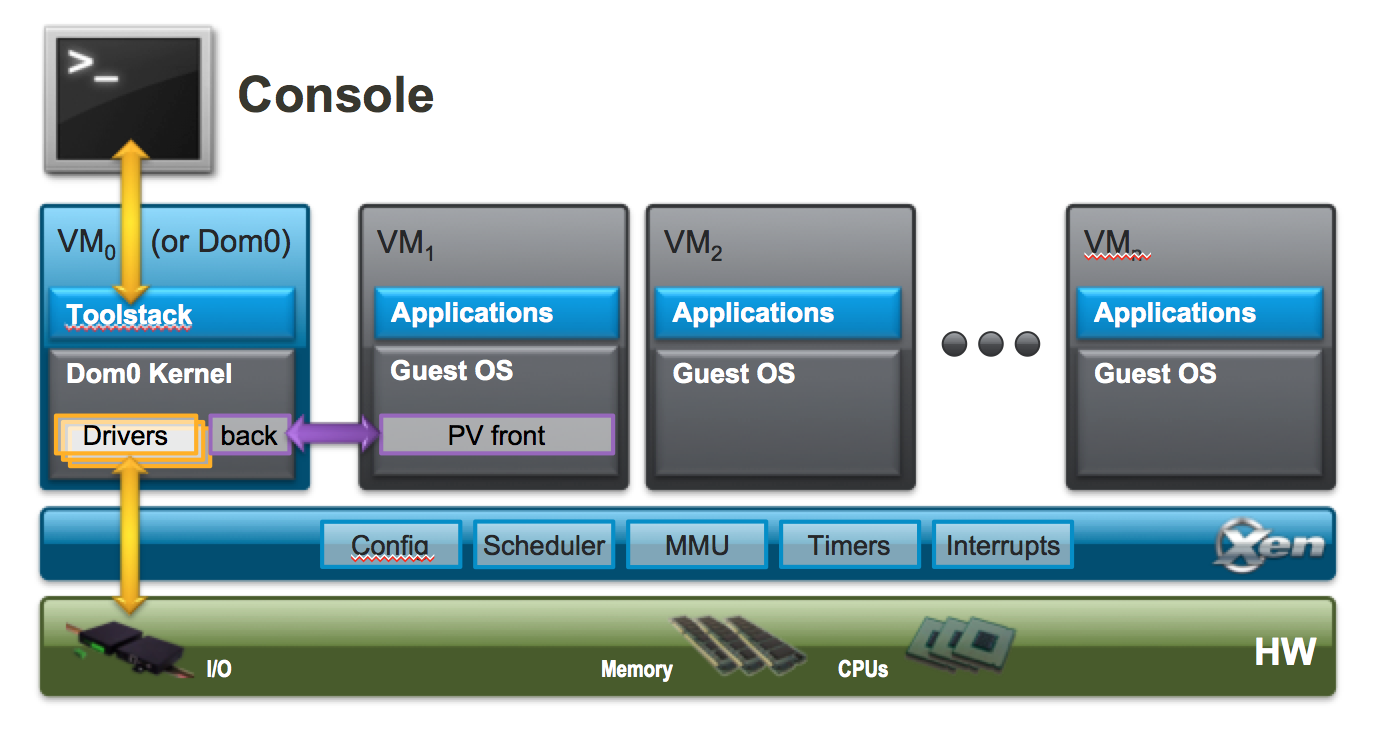
\includegraphics[width=0.60\hsize]{Xen_Arch_Diagram.png}
\caption{Xenin arkkitehtuurikaavio\cite{xen_overview}.}
\label{kuva_xen}
\end{figure}

\subsubsection{KVM}
%http://www.linuxthoughts.com/?p=110
%https://www.youtube.com/watch?v=6n-ANRWqll8
KVM (Kernel Mode Virtualization) on Linux-ytimeen rakennettu tuki virtualisoinnille. KVM vaatii prosessorilta virtualisointituen. KVM ei itsessään emuloi mitään, vaan tarjoaa käyttäjätasolle rajapinnan prosessorin virtualisointiominaisuuksiin. KVM on toteutettu siten, että se muuttaa Linux-ytimen hypervisoriksi hyödyntäen muita Linuxin komponentteja, kuten vuorottelijaa ja muistinhallintaa, kuvan \ref{kuva_kvm} mukaisesti. \citep{kvm1}

% http://www.linux-kvm.org/wiki/images/6/61/KvmForum2007$kf2007-keynote.pdf
KVM:n kehitys alkoi vuonna 2006 \cite{kvm3}. Ensimmäinen vakaa, Linuxin ytimen mukana toimitettava versio julkaistiin syyskuussa 2012. KVM koostuu ydinmoduulista kvm.ko, joka toteuttaa virtualisoinnin perusrakenteet, prosessoririppuvaisista ydinmoduuleista (esim. kvm-intel.ko ja kvm-amd.ko.) ja käyttäjätason ohjelmasta (qemu-system-ARCH), joka emuloi laitteiston ja toteuttaa virtuaalikoneiden (guest) hallinnan. Jokaiselle virtuaalikoneelle emuloidaan omat laitteistot. Alussa hallintaan käytettiin muunneltua QEMU:n versiota, mutta QEMU 1.3:sta lähtien tarvittavat muutokset on lisätty QEMU:un. KVM:lle ei toistaiseksi ole toteutettu muita käyttäjätason hallintaohjelmia kuin QEMU. QEMU:n päälle on kuitenkin toteutettu laaja joukko hallintaohjelmia (libvirt) \cite{kvm2}. KVM on yksi harkinnanarvoinen virtuaalikone, jos ajoneuvotietokoneen alkuperäinen käyttöjärjestelmä täytyy saada virtualisoitua.


%https://www.suse.com/documentation/sles-12/book_virt/data/sec_kvm_intro_arch.html
\begin{figure}[H]
\centering
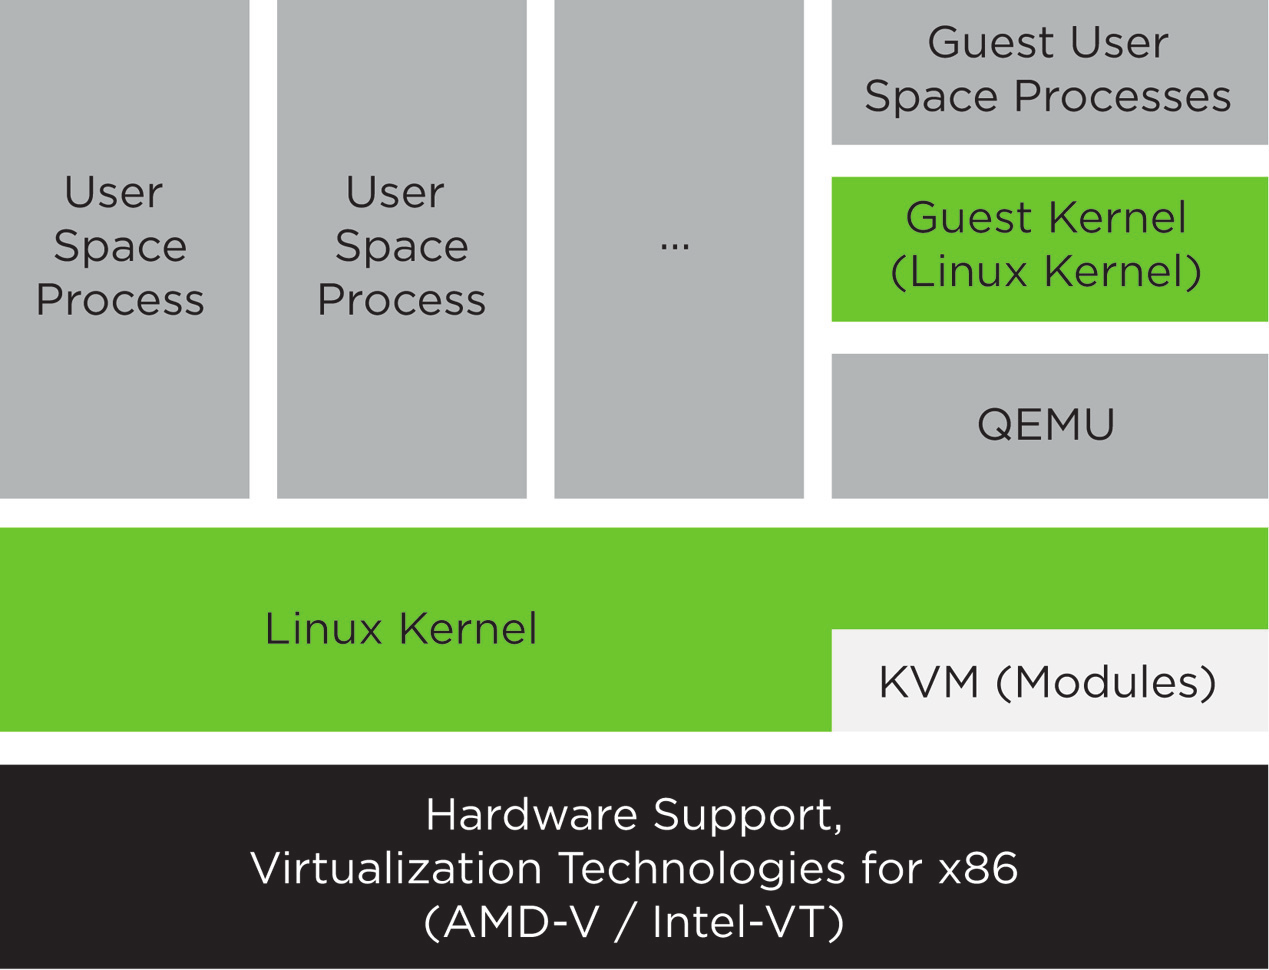
\includegraphics[width=0.60\hsize]{kvm_qemu.png}
\caption{KVM:n arkkitehtuurikaavio\cite{kvm4}.}
\label{kuva_kvm}
\end{figure}

\subsubsection{Oracle Virtualbox}
Oracle Virtualbox on henkilökohtaisessa käytössä ilmainen virtuaalikone Windows- ja *NIX-käyttöjärjestelmille. Se toimii 2-tason hypervisorina (käyttöjärjestelmän päällä suoritettavana virtuaalikoneena) ja tukee x86- ja x64-käyttöjärjestelmien virtualisointia \cite{virtualbox_manual}. Virtualboxin perusohjelmisto on GPLv2-lisensoitua, ja siihen tarjotaan  PUEL-lisensoituja suljetun lähdekoodin lisäpaketteja. Virtualboxin ensimmäinen versio julkaistiin 15.1.2007 yrityksen Innotek toimesta. Sun Microsystems osti Innotekin helmikuussa 2008. Oracle Corporation osti Sun Microsystemsin 27.1.2010 ja vastaa nykyisin Virtualboxin myynnistä ja kehityksestä.


%With version 4 of VirtualBox, released in December 2010, the core package is free software released under GNU General Public License version 2 (GPLv2). This is the fully featured package, excluding some proprietary components not available under GPLv2.
%https://www.virtualbox.org/wiki/VirtualBox_PUEL
%https://www.virtualbox.org/wiki/Licensing_FAQ
%Personal use is when you install the product on one or more PCs yourself and you make use of it (or even your friend, sister and grandmother). It doesn't matter whether you just use it for fun or run your multi-million euro business with it. Also, if you install it on your work PC at some large company, this is still personal use. However, if you are an administrator and want to deploy it to the 500 desktops in your company, this would no longer qualify as personal use. Well, you could ask each of your 500 employees to install VirtualBox but don't you think we deserve some money in this case? We'd even assist you with any issue you might have.

Virtualbox on ilmainen koti- ja arviointikäyttöön. Oracle myy Enterprise-versiota noin 50 euron hintaan (minimitilausmäärä 100 kappaletta).
Virtualboxin PUEL-lisenssin mukaan Virtualboxin ilmaisen version käyttö on sallittua kaupallisesti, jos ohjelmiston asennus ja käyttö on yksittäisen henkilön hallittavissa. Maksullinen Enterprise-versio tarvitaan, jos ohjelmistoa toimitetaan esiasennettuna tai sen asennusta ja käyttöä vaaditaan tai hallitaan yritystasolla.\citep{virtualbox_puel,virtualbox_licensing}

Virtuaalikoneita hallitaan ja Virtualboxin graafisella käyttöliittymällä että VBoxManage-komentoriviohjelmistolla, joka tarjoaa graafisen käyttöliittymän ominaisuuksien lisäksi pääsyn kaikkiin virtualisointimoottorin ominaisuuksiin \cite{virtualbox_manual}. Virtualboxin ominaisuuksiin kuuluu virtuaalikoneiden moniprosessorituki, USB-laitteiden tuki ja snapshotit. Virtualbox tukee kahden sarjaportin välittämistä kohdejärjestelmälle. Lisäksi VirtualBoxista on olemassa versiont Windows-, Linux-, OSX-, (Open)Solaris- ja FreeBSD-käyttöjärjestelmille. Virtualboxin puutteita ovat rajoittunut virtuaalikoneiden verkonhallinta useiden virtuaalikoneiden tapauksessa, USB 3.0-tuen puuttuminen ja sisäkkäisten virtuualikoneiden suorituksen tuki \cite{vplayervsvbox}. Ajotietokoneen virtualisointia ajatellen Virtualbox on yksi harkinnanarvoinen ohjelmisto toteutukseen.


\subsubsection{VMWare Player}
VMWare Player on VMWaren vuonna 2008 julkaistu kaupallinen virtualisointiohjelmisto. Uusin versio on joulukuussa 2014 julkaistu 7.0. VMWare Player on kotikäyttöön ilmainen, mutta kaupallinen käyttö vaatii lisenssin hankkimisen. VMWare Player käyttää samaa virtualisointiydintä VMWare Workstationin kanssa, josta riisuttu versio Player oikeastaan on. VMware Playerin ominaisuuksiin kuuluu neljän sarjaportin välitys kohdejärjestelmälle. Laitteiston välitystuki Playerissa on hyvä. VMware Playerista on versiot Windows- ja Linux-käyttöjärjestelmille. \citep{vmware1}


Playerista puuttuvat snapshotit, ja siinä on hyvin rajoittunut komentorivi-käyttöliittymä. Suoritusnopeudessa VMware Player voittaa Virtualboxin pienellä erolla \cite{vplayervsvbox}. VMware Player on Virtualboxin kannsa ominaisuuksiltaan muuten hyvin tasaväkinen, mutta maksullinen, mistä syystä Player jätettiin pois harkinnanarvoisista virtuaalikoneohjelmistoista ajoneuvotietokoneen virtualisoimiseksi.




% \subsubsection{KVM Hosting}
% %Here QEMU deals with the setting up and migration of KVM images. It is still involved in the emulation of hardware, but the execution of the guest is done by KVM as requested by QEMU.
% QEMU hoitaa virtualisoinnin KVM:n avulla. QEMU emuloi tarvittavat laitteet ja KVM hoitaa itse virtualisoinnin.

% \subsubsection{Xen Hosting}
% %QEMU is involved only in the emulation of hardware; the execution of the guest is done within Xen and is totally hidden from QEMU.
% Xeniä käytettäessä QEMU hoitaa ainoastaan laitteistoemuloinnin, itse virtuaalikoneen suoritus tapahtuu Xenin kautta eikä QEMUlla ole siihen pääsyä.

\subsubsection{Windows Virtual PC}
Windows Virtual PC on Microsoftin ilmaiseksi tarjoama virtuaalikone Windows 7 -käyttöjärjestelmälle. Uusin versio on 6.1, jonka tuettuina kohdekäyttöjärjestelminä ovat Windows XP, WIndows Vista, ja Windows 7. \citep{vpc_tips}

Connectix kehitti Virtual PC:n Machintonin System 7.5 -käyttöjärjestelmälle vuonna 1997. Windows-versio julkaistiin vuonna 2001. Microsoft osti Virtual PC:n Connectixilta vuonna 2003. Vuonna 2006 Microsoft julkaisi Virtual PC 2004 SP1:n ilmaiseksi. Vuonna 2009 Virtual PC:n nimi vaihdettiin Windows Virtual PC:ksi, joka tukee ainoastaan Windows 7:ää ja sen jälkeen julkaistuja Windowseja. Virtual PC:n asettamat käyttöjärjestelmärajoitukset sulkevat sen pois mahdollisten virtuaalikoneiden listalta.


\section{Järjestelmäemulointi}
Järjestelmäemuloinnissa alkuperäisiä ohjelmistoja ja käyttöjärjestelmää suoritetaan emulaattorissa toisen järjestelmän päällä. Emuloimalla saavutetaan laitteistoarkkitehtuuririippumattomuus isäntäkoneen ja emuloitavan järjestelmän välillä. Emuloinnin haittapuolena on hitaus. Nyrkkisääntönä on 20 \%:n hyötysuhde \cite{tinycc}, kun parhaat emulaattorit pääsevät noin 40-80 \%:n hyötysuhteeseen. \citep{40pperf}

Hitauden vuoksi emulointi ei ole erityisen suotuisa vaihtoehto huomattavasti nopeampaan virtualisointiin verrattuna. Työssä käytettävät ohjelmat eivät kuitenkaan ole mitenkään resurssisyöppöjä, joten emulointia voi ajatella varteenotettavana vaihtoehtona, jotta työssä voidaan mahdollisesti käyttää x86-arkkitehtuurin lisäksi muita prosessoriarkkitehtuureita, joista ARM on laajan suosionsa takia vaihtoehtojen kärjessä.

% Blaah. Esittely QEMUsta, Virtualboxista, VirtualPC:stä, VMWaren shaibasta
%http://qemu.weilnetz.de/qemu-tech.html#intro_005ffeatures
\subsubsection{QEMU}
QEMU (Quick Emulator) on avoimen lähdekoodin emulaattori ja virtuaalikone, joka toimii Linuxin lisäksi myös Windowsissa ja Mac OS X:ssä. QEMU tukee erilaisia toimintamoodeja. QEMU:n rakenne on jaettu taustajärjestelmään, joka vastaa isäntäkoneen arkkitehtuurituesta, ja edustaohjelmaan, joka vastaa kohdeprosessorin emuloinnin toteuttamisesta. Tällä rakenteella on saatu aikaiseksi järjestelmä, joka on helppo kääntää ja laajentaa uusille prosessoreille ja niiden käskykannoille. \citep{qemu_doc}

Järjestelmäemuloinnissa QEMU emuloi koko tietokoneeen, mukaan lukien laitteistot. Kun kohdejärjestelmää emuloidaan, arkkitehtuurin ei tarvitse olla sama kuin isäntäkoneella. QEMUun on toteutettu suhteellisen laaja määrä erilaisia laitteita, kuten 11 erilaista USB Hostia, 8 erilaista verkkokorttia, 5 erilaista näytönohjainta ja 8 äänikorttia \cite{qemu_doc}. QEMU:ssa on käytetty GIL:ä (Global Interpreter Lock) synkronoimaan suoritusta, joten se suorittaa järjestelmäemuloinnin yksisäikeisesti, vaikka kohdejärjestelmälle olisikin toisin väitetty \cite{qemu_tech}

%http://qemu.weilnetz.de/qemu-tech.html#QEMU-compared-to-other-emulators
QEMU käyttää dynaamista käännöstä (dynamic translation) nopeuttakseen emulointinopeutta. Dynaamisessa käännöksessä tulkitaan ja käännetään suoritettavaa tiedostoa pieni osa, blokki, kerrallaan. Blokki on haarautumiseen ja hyppykäskyihin asti oleva pätkä käskyjä. Koska yleensä dynaamiset kääntäjät ovat monimutkaisia ja arkkitehtuurisidonnaisia, on QEMU:n kääntäjä TCG (Tiny Code Generator) pidetty yksinkertaisena ja helposti siirrettävänä. TCG:n perusajatus on jakaa jokainen käsky TCG:n RISC-tyyppisiksi käskyiksi, jotka sitten muutetaan kohdejärjestelmän käskyiksi. \citep{qemu_tech}


\subsubsection{Bochs}
Bochs on pelkästään x86-arkkitehtuuriin keskittynyt avoimen lähdekoodin emulaattori. Sen ensimmäinen versio julkaistiin vuonna 1994, jolloin se oli vielä kaupallinen tuote. Vuonna 2000 Mandrakesoft (ranskalainen yritys, joka on erikoistunut Linuxiin) osti Bochsin sen kehittäjältä Kevin Lawtonilta ja julkaisi lähdekoodit LGPL-lisenssillä \cite{bochs0}. Bochsia käytetään käyttöjärjestelmäkehityksessä apuna, ja se sisältääkin emuloinnin 8-ytimiselle prosessorille ja kehittyneet vianetsintätyökalut. \citep{bochs_doc}

Bochs tukee sarjaportin välitystä isäntäkäyttöjärjestelmän ja emuloidun koneen välillä, ja se pystyy emuloimaan alkuperäisen ajoneuvotietokoneen käytössä ollutta Windows 98-käyttöjärjestelmää, joten Bochsia pystyisi siten käyttämään emulaattorina tässä työssä. QEMUun verrattuna Bochsin käyttö ei kuitenkaan tuo mitään ylimääräistä arvoa vaihtoehtona, joten en suosittele sen käyttöä tässä tarkoituksessa.


\section{Ohjelmistojen emulointi}
Ohjelmistojen emuloinnilla tarkoitetaan käyttäjätilan emulointia, jossa voidaan suorittaa kohdejärjestelmän ohjelmia suoraan ilman, että emuloidaan koko tietokone käyttöjärjestelmineen väliin. Tämä onnistuu tietyillä ohjelmilla tiettyjen ohjelmistoarkkitehtuurien välillä \cite{tinycc, qemu_use}. Vaihtoehdolla voi suorittaa muun muuassa x86-ohjelmia ARM-prosessoreilla.

\subsubsection{QEMU}
QEMU tarjoaa virtualisoinnin ja laitetason emuloinnin lisäksi myös käyttäjätilan emulointia Linux-, OSX- ja BSD-käyttöjärjestelmissä \cite{qemu_use}. Tuettuja kohdeprosessoriarkkitehtuureita ovat x86 (i386), ARM, M68K ja SPARC.

Käyttäjätilan emuloinnissa QEMU suorittaa järjestelmäkutsujen ja I/O-kutsujen tulkkauksen, joka korjaa myös mahdolliset tavujärjestys- ja 32/64-bittisyydestä aiheutuvat ongelmat. Linuxin signalointi pystytään suurimmaksi osaksi hoitamaan suoraan isäntäkoneelle. Vain signaalinkäsittelyn signaalit signaalien tutkimiseen (sigaction) ja signaalinkäsittelijästä poistumisen (sigreturn) on tarvinnut emuloida. Lisäksi järjestelmäkutsuista uusien säikeiden luonti on hoidettu tekemällä jokaista säiettä varten uusi virtuaaliprosessori. \citep{qemu_tech}

QEMU:lla onnistuu oman dokumentaationsa mukaan myös Wine-yhteensopivuuskerroksen emulointi, jota tarvitaan, jotta Windows-ohjelmat, kuten ajoneuvotietokoneen ohjelmista Motomit, saadaan suoritettua myös muilla arkkitehtuureilla \cite{qemu_use}. QEMUn käyttäjätilan emulointi vaikuttaakin tutustumisenarvoiselta ominaisuudelta tässä varsin monipuolisessa virtualisointi- ja emulointiohjelmistossa.


%http://eltechs.com/product/exagear-desktop/
%http://magazine.odroid.com/assets/201502/pdf/ODROID-Magazine-201502.pdf
\subsubsection{Eltechs ExaGear Desktop}
Eltechs ExaGear Desktop on kaupallinen toteutus Linuxille 32-bittisten x86-ohjelmien suorittamiseksi ARMv7-arkkitehtuurin prosessoreilla. Ohjelmisto julkaistiin lokakuussa 2014. Se on omien testiensä perusteella viisi kertaa QEMU:a nopeampi \cite{eltechs:exagear}. SysBenchín synteettisten testien perusteella ExaGear Desktopin suoritusnopeus on 50--85 \% natiivista nopeudesta.

ExaGear Desktop ei sisällä grafiikan laitteistokiihdytystukea, joten OpenGL/DirectX Winellä vaativat ohjelmistot suoritetaan ohjelmistorenderöijällä. Tämä on hidasta, eikä ohjelmistorenderöijä tue kaikkia OpenGL-standardin ominaisuuksia. Lisäksi on raportoitu ongelmista äänentoistossa, jos ääntä tuotetaan useasta lähteestä yhtäaikaa. Ajoneuvotietokoneen tarpeita ajatellen nämä puutteet eivät haittaa, koska käytettävät ohjelmat eivät tarvitse 3D-kiihdytystä eivätkä ääniä. \citep{eltechs:odroid}

% Caveats
% There are some quirks with ExaGear that make things a little bit harder to use. For example, the file access in the ExaGear
% environment is somewhat slow. Starting TeamViewer can take anywhere from 30 seconds up to a minute on an
% ODROID-U3, which happens regardless of whether you’re using an eMMC module or SD card. You should occasionally
% run “apt-get update” in your ExaGear environment in order to update the package lists, or else some packages may not be
% installed during the TeamViewer or Skype installation. If you perform a system update using “apt-get upgrade” and/
% or “apt-get dist-upgrade” command, you might encounter several issues, since the image was highly modified. I noticed that
% a few things were forgotten, such as altering the initramfs-tools to disable the creation of an initrd.img file, which isn’t possible
% anyway. Also, some packages will fail to update, which requires some Linux expertise to fix, but an upgrade is probably not really
% necessary once everything is working. Another issue is that ExaGear distributes tasks over all CPU
% cores, which is generally a very good thing since it uses all the power it can get, but it also can lead to a very hot CPU if an
% application uses a lot of CPU power. For example, I was running a Windows application called Blender on my XU3 using
% ExaGear and Wine, which resulted in all 8 cores running at 100%, and even with the fan spinning at its maximum speed,
% the temperature rose to over 94°C (200°F)! Overall, I really like what you can do with ExaGear, and
% although I was very skeptical when it was first announced, I have to say it’s doing a very good job.

% Wine
% If you use ExaGear with Wine, a very convenient program is PlayOnLinux, which allows you to easily configure and install
% Windows applications under Wine. If you try to run fullscreen applications such as games using Wine, you need to configure
% Wine to run in a fake desktop with a size of 800x600 or 1024x768, rather than allow it to run natively in Linux. PlayOnLinux
% may spare you some of these resolution problems, especially with the C1, which cannot change resolutions on the fly.
% PlayOnLinux also makes recovery easier when a program hangs, since it is able to actually close the specific program


%\lipsum[1-5]

\newpage

\chapter{Ajoneuvotietokoneiden lainsäädäntö ja standardit}

Lain ja olosuhteiden asettamia vaatimuksia ajoneuvotietokoneelle käsitellään seuraavissa direktiiveissä ja standardeissa:

CEN EN55022 -standardi määrittää kevyen teollisuuden laitteiden ja tietokonelaitteiden säteilypäästöjen raja-arvot ja määrittää, miten mittaus tulee suorittaa. Standardissa laitteet on jaoteltu kahteen luokkaan, A ja B, joista B-luokan laitteet ovat paremmin suojattuja. \citep{EN55022}

EU-direktiivi 2004/104/EY (Autoteollisuuden EMC-direktiivi) määrittää, että 1.7.2006 alkaen valmistettujen ajoneuvojen ja kiinteästi asennetun ajoneuvoelektroniikan aiheuttamat säteilypäästöt ja päästöjen sietokyky mitataan direktiivin mukaisesti. Direktiiviin on julkaistu lisäys 2005/83/EY, joka tarkentaa direktiiviä. Uusi direktiivi korvaa aiemman direktiivin 95/54/EY.

Uusi direktiivi vaatii tyyppihyväksynnän vain laitteilta, joilla on
vaikutusta ajoneuvon hallintaan, kuljettajan asennon muuttamiseen tai
kuljettajan näkyvyysalueeseen. Laitteiden, joiden ei tarvitse olla
tyyppihyväksyttyjä, pitää täyttää kuitenkin EMC-direktiivin 89/336/ETY
tai radio- ja telepäätelaitedirektiivin 1999/5/EY vaatimukset. \citep{1999/5/EY,89/336/ETY}

EMC-direktiivi 89/336/ETY määrittelee ainoastaan laitteistolta vaadittavat ominaisuudet sähkömagneettisen yhteensopivuuden takaamiseksi. Direktiivin tarkoitus on ohjeistaa valmistajia tekemään elektromagneettisesti yhteensopivia laitteita. Direktiivi koskee kaikkia sähkölaitteita ja -asennuksia, joita ei direktiivissä ole erikseen rajattu sen ulkopuolelle \cite{89/336/ETY}. Direktiivi 2004/108/EY kumosi vanhemman direktiivin 89/336/ETY 20.7.2004 alkaen. 2004/108/EY  erotteli kiinteille asennuksille ja laitteille tehtävät asennukset ja yksinkertaisti vaatimustenmukaisuuden arviointimenettelyä. \citep{2004/108/EY}

Radio- ja telepäätelaitedirektiivi 1999/5/EY määrittää radio- ja telepäätelaitteiden yhteensopivuuden Euroopan laajuisesti. Kaikkiin direktiivin piiriin kuuluvien laitteiden tulee olla turvallisia käyttäjälle ja muille henkilöille ja täyttää vaaditut suojavaatimukset sähkömagneettisen yhteensopivuuden osalta. Lisäksi
direktiivi määrittää, että laitteistojen tulee olla rakennettuja siten, että ne käyttävät tehokaasti radioviestintään varattua spektriä ja resursseja. Tietyille laiteluokille on lisäksi määritelty vielä muita vaadittuja lisäominaisuuksia, kuten yksityisyyden suojan takaaminen, yhteensopivuus muiden laitteistojen välillä, petoksia ehkäisevien ominaisuuksien sisältäminen, tuki hätäpalveluihin pääsyn takaaville ominaisuuksille ja/tai ominaisuudet, joilla laitteistojen
käyttö tehdään helpommaksi vammaisille \cite{1999/5/EY}. Direktiivi 1999/5/EY on kumottu 13.6.2016 alkaen direktiivillä 2014/53/EU radiolaitteiden asettamista saataville markkinoilla koskevan jäsenvaltioiden lainsäädännön yhdenmukaistamisesta. \citep{2014/53/EU}

IP-suojaluokitus on standardissa IEC 60529 määritetty järjestelmä sähkölaitteiden tiiveyden määrittämiseksi. IP-luokitus kertoo laitteiden suojauksen pölyä ja vettä vastaan \cite{IEC60529}. IP54-suojaluokitetut tuotteet ovat pölysuojattuja (ei täydellistä tiiviyttä, mutta ei pölykertymiä) ja roiskesuojattuja.

IP67/66-suojaluokitetut tuotteet ovat täysin pölytiiviitä ja kestävät suurella paineella tulevan vesiruiskun. IP67/66-tuotteet kestävät tärinää ja iskuja 5M3-vaatimusten mukaisesti. (DIN EN 60721-3-5, MIL-STD 810F.) Kuten aiemmin mainittiin, nykyisessä järjestelmässä Nero täyttää EN55022-standardin vaatimukset ja on IP54-suojattu. Uuden valmiina hankittavan järjestelmän tulisi täyttää EN55022-standardin ja direktiivin  2004/104/EY vaatimukset.

\newpage
\chapter{Tehdyt tutkimukset ja huollot}

\section{Tutustuminen Nero-ajoneuvotietokoneeseen}
Ensimmäisen kerran tutustuin Sunitin Nero-ajoneuvotietokoneeseen toukokuussa 2014, kun työn kohteena olevasta yksilöstä oli rikkoutunut kiintolevy. Tällöin tutkin ja selvitin tietokoneen ominaisuudet, liitännät ja ohjelmistot. Koska ohjelmistot olivat saatavana kopioina Motomit-jälleenmyyjältä ja Valmetilta, ei alkuperäistä kiintolevyn sisältöä tarvinnut saada talteen. Tietokoneeseen hankittiin käytetty Hitachin 40 Gb 2,5" IDE -kiintolevy, asennettiin käyttöjärjestelmä (Windows 98) ja ohjelmistot valmiiksi virtuaalikoneessa ja varmuuskopioitiin asennus. Lopuksi 1.7.2014 testattiin toimivuus tuotantoympäristössä.

Ensimmäisessä huollossa vaihdettu kiintolevy rikkoontui vain muutaman kuukauden käytön jälkeen. Koska kiintolevyn koolla ja nopeudella ei ole tässä tietokoneessa erityisemmin väliä, valittiin uudeksi kiintolevykorvikkeeksi paremmin tärinää ja vaihtelevia lämpöolosuhteita kestävä SD-IDE-muistikorttiadapteri ja 2 Gb:n muistikortti. Alkuperäinen SecureDigital-standardi mahdollistaa vain 2 Gb:n kapasiteetin ja väylän maksiminopeuden 12,5 Mb/s (kirjoitusnopeus on huomattavasti vähemmän, noin 1--2 Mb/s ). \citep{sd:2gb}

Huhtikuussa 2015 Nero-ajoneuvotietokoneesta rikkoontui BIOS:n CMOS-asetuksia ylläpitänyt NiMH-akku, minkä seurauksena ajoneuvotietokone kadottaa asetuksensa aina päävirtojen katkaisun yhteydessä. Kiintolevy pitää erikseen etsiä jokaisen päävirran katkaisun jälkeen BIOS:sta, mikä tekee tietokoneen käytön hankalaksi tai jopa mahdottomaksi hakkuukoneen kuljettajalle. Akkupaketin NiMH-kennot uusittiin ja BIOS-asetukset määritettiin uudelleen, jolloin kone saatiin taas takaisin käyttöön.

\section{Valitun toteutustavan perustelut}
Saatavissa olevista laitteistoista ja alkuperäisten ohjelmistojen arkkitehtuurista päädyin valitsemaan testaukseen X86-arkkitehtuurilla ja Linux-käyttöjärjestelmällä toteutettavan kokonaisuuden, jossa on asennettuna Winen, Dosboxin ja Dosemun päälle tarvittavat Motomit- ja Terman-ohjelmat. Lisäksi asensin virtuaalikoneeseen (Virtualbox) alkuperäisen Windows 98 -käyttöjärjestelmän ja alkuperäiset ohjelmat kokeiltavaksi. Näin sain kokeiltua Linuxin ja virtualisoinnin sopivuuden varsinaisen uuden ajoneuvotietokoneen mahdollisiksi toteutustavoiksi.

Linux valittiin kohdekäyttöjärjestelmäksi, koska Windows tiedetään Motomitin osalta toimivaksi vaihtoehdoksi (Motomitistä on olemassa Windows 7 -yhteensopiva versio). DOS-ohjelmia ei voi suorittaa suoraan Windowsista, sillä vaikka myös Windowsin 32-bittisistä versioista löytyy ''Virtual DOS machine'',  se ei rajoita ohjelmien suoritusnopeutta eikä tue suorayhteyttä sarjaväylälle, minkä takia lähes kaikissa toteustavoissa tarvitaan jokin lisäohjelma, jotta sarjaportti saadaan toimimaan DOS:n puolella. Dosboxista on olemassa Windows- että Linux-versiot, minkä takia yhteensopivuuden pystyy testaamaan alustavasti Linuxin avulla. Päätökseen valita Linux vaikutti myös vahvasti oman osaamisen ja mieltymysten painottuminen Linux-puolelle. En siis nähnyt erityistä estettä olla kokeilematta järjestelmän toimivuutta Linux-käyttöjärjestelmässä.

Muita mahdollisia vaihtoehtoja toteutukselle olisi ollut X86-pohjainen Windows 7 tai Windows 8 -käyttöjärjestelmällä varustettu kannettava. Tätä ratkaisua ei käytetty, koska haluttiin kartoittaa käytettävien ohjelmien toiminta myös Linux-puolella, ja testaukseen käytetystä tietokoneesta puuttui tarvittava Windows-lisenssi.

ARMv7-pohjaisista tietokoneista, kuten Raspberry Pi 2 ja BeagleBone Black, voisi yhdessä Eltechs ExaGear Desktop x86 -tulkkausohjelmiston kanssa rakentaa kevyen ajoneuvotietokoneen. Tämä vaihtoehto ei kuitenkaan ollut vielä insinöörityön selvitysvaiheessa tiedossa, vaan tuli esille vasta helmikuussa 2015, kun Raspberry Pi 2 julkaistiin. Koska itse tehty järjestelmä olisi vaatinut huomattavasti enemmän suunnittelua, rakentelua ja testausta, todettiin ratkaisu tällä aikataululla liian työlääksi ja epävarmaksi. Kuten sanottu, nykyinen ajoneuvotietokone osoittautui vielä korjattavissa olevaksi. Nykyisen järjestelmän korvaavista vaihtoehdoista kerron tarkemmin luvussa \ref{ch:korvaava_jarjestelma}.

\section{Käytetyt laitteistot ja ohjelmat}
\subsubsection{Käytetyt laitteistot}
Testaukseen käytettiin vanhaa Fujitsu-Siemensin Amilo Pa 2510 -kannettavaa tietokonetta vuodelta 2007. Amilo Pa 2510:ssa on AMD Turion 64 X2 TL-50 1.6 GHz -prosessori, ATI Radeon Xpress X1200 128 Mb -näytönohjain, 2 Gb keskusmuistia, 15,4'':n näyttö ja 120 Gb:n kiintolevy. Testauskoneen tehot riittävät hyvin ohjelmistojen testaukseen ja virtuaalikoneen kanssa että emuloituna ja ohjelmistorajapinnan kautta \cite{fs_amilo:review}. Puutteena tietokoneessa on sarjaporttien puute ja rikkoutunut näppäimistö.

Sarjaporttiliittimet ovat poistuneet kannettavista USB:n yleistyttyä jo 2000-luvun alussa, vaikka vielä on myynnissä yrityskäyttöön tarkoitettuja kannettavia tietokoneita, joissa on vähintään yksi natiivi sarjaporttiliitin \cite{hp:laptop}. Sarjaportin puuttuminen korvataan tässä tapauksessa USB-sarjaporttiadapterilla, jonka avulla kannettavaa tietokonetta voidaan käyttää testaukseen.

Rikkinäinen näppäimistö korvataan erillisellä USB-väylään liitettävällä näppäimistöllä testauksen ajaksi. Sähkönsyöttö testauksen ajan hoituu kannettavan omalla akulla, jossa on vielä kapasiteettia pitää kannettava käynnissä testauksen ajan.

Käytettävä USB-sarjaporttiadapteri oli eBaystä testaukseen hankittu 2-porttinen Unitek USB to Dual Serial Cable Y-106 \cite{serial:unitek}. Y-106-adapteri käyttää MosChip Semiconductorin MCS7820-piiriä muunnokseen. Adapteri valittiin, koska siinä oli tarvittavat 2 sarjaporttia, sen myyntihinta oli edullinen (n. 25 € sisältäen toimituksen) ja käytetylle muunninpiirille on ajurituki sekä Windows- että Linux-käyttöjärjestelmille.


\subsubsection{Käytetyt ohjelmat}
Xubuntu 14.04 on Ubuntu 14.04:ään perustuva (joka taas on Debianiin perustuva) Linux-distro, jossa käyttöliittymäksi on vaihdettu XFCE 4.10 ja mukana toimitettavista ohjelmistoista on valittu kevyemmät versiot kuin Ubuntussa \cite{xubuntu:about}. Xubuntu valittiin käyttöjärjestelmäksi, koska testaamiseen käytettävä kannettava oli hieman vanhempi ja Xubuntu on todettu jo aiemmin toimivaksi käyttöjärjestelmäksi kyseisessä tietokoneessa.

Käyttöjärjestelmäksi valittiin Xubuntusta pitkän tuen versio 14.04. Xubuntu asennettiin oletusasetuksilla testikoneeseen. Lisäksi Xubuntu laitettiin kirjautumaan sisään automaattisesti, ja Dosbox ja MotomitPC laitettiin käynnistymään automaattisesti sisäänkirjautumisen yhteydessä.

Wine on Windows-yhteensopivuuskerros Unixin kaltaisiin (mm. Unix/Linux/OS X/Solaris) käyttöjärjestelmiin, ja se mahdollistaa Windows-ohjelmien käyttämisen käytetyssä käyttöjärjestelmässä. Wineä tarvitaan, jotta apteeraukseen käytettävä Motomit PC -ohjelmisto saadaan toimimaan Linuxissa. Vaikka Motomit sisältääkin taustajärjestelmänään Linuxin \cite{motomit:manual}, on käyttöliittymänä toimivasta Motomit PC -ohjelmasta olemassa vain Windows-versio.

Dosbox on DOS-emulaattori, joka emuloi IBM PC -yhteensopivaa tietokonetta 286/386-prosessorilla ja monia muita saman aikakauden laitteistoja. Dosbox sisältää lisäksi suoratuen sarjaportille, minkä takia se valittiin käytettäväksi DOS-emulaattoriksi. Dosboxia tarvitaan, että Terman-ohjelmisto saadaan toimimaan uudemmissa Windowseissa ja Linuxeissa.

Dosemu on virtuaalikone ja DOS-rajapintakerros Linuxille, ja se mahdollistaa DOS-ohjelmien suorittamisen x86-arkkitehtuuria käyttävässä Linux-käyttöjärjestelmässä. Dosemu valittiin myös testattavaksi vaihtoehdoksi Termanin saamiseksi toimimaan Linux-käyttöjärjestelmässä.

\section{Asennus ja asetusten säätö}
Käytetylle USB-sarjaporttiadapterille lisättiin oma udev-sääntö, jonka ansiosta adapterin kaksi sarjaporttia tulevat näkyviin Linuxissa samoilla laitetiedostonimillä (Device file), vaikka tietokoneeseen olisi kytkettynä useampi erilainen USB-sarjaporttiadapteri.

Jotta sarjaportit saa toimimaan Winessä Windowsin käyttämillä COM-porttinimillä Windows-ohjelmien puolella, tulee laitetiedostoista tehdä symboliset linkit ''\textasciitilde{}/.wine/dosdevices/''-hakemistoon halutuilla nimillä (COM1 ja COM2) \cite[s. 21]{wine:manual}.

Dosboxin ja Dosemun asetuksiin tuli määrittää käytettävät sarjaportit. Lisäksi Dosboxista muutettiin suoritusnopeutta ja näytön kokoa suuremmaksi, jotta käytettävyys olisi parempi \cite{dosbox:conf}. Molemmat ohjelmat jätettiin ikkunointimoodiin, jotta yhteiskäyttö Motomit PC:n kanssa olisi helpompaa.

%Xubuntu ohjattiin kirjautumaan automaattisesti oletuskäyttäjätunnuksilla sisään käynnistysvaiheessa. Ohjelmat laitettiin käynnistymään automaattisesti sisäänkirjautumnisen yhteydessä (lisäksi tarvittiin vielä Dosboxiin ja Dosemun AUTOEXEC.BAT -tiedostoon lisätä Terman käynnistymään automaattisesti). Kun asetukset oli säädetty toimimaan, asetetaan tiedostojärjestelmä vain luku-tilaan, jotta saadaan parannettua kokoonpanon luotettavuutta.

\section{Simple Serial Repeater -ohjelmisto}
Simple Serial Repeater (SRPT) on ohjelmisto sarjaliikenteen tallentamiseen ja toistoon. Sen tarkoitus on mahdollistaa sarjaliikenteen helppo tallennus ja toisto ja virtuaalisille että fyysisille sarjaporteille. SRPT kehitettiin testauksen avuksi, jotta pystyttiin testaamaan tiedonsiirron toimivuus, ilman että testausta tarvitsisi mennä tekemään joka kerralla työn kohteena olevan moton luokse. Tässä tarkoituksessa SRPT toimikin hyvin, ja projektin edetessä pantiin merkille muutamia kehitysideoita, joilla testaustyökalua saataisiin vielä monikäyttöisemmäksi.

SRPT on tarkoituksella pidetty suhteellisen yksinkertaisena, mutta tarvittaessa helposti laajennettavana. Ohjelmiston jako useisiin ohjelmiin ja käytettävä tiedostomuoto tukevat tätä. Ohjelmisto on pidetty tarkoituksella komentorivipohjaisena, koska graafiselle käyttöliittymälle ei ole nähty tarvetta.

SRPT on ohjelmoitu Python 2 -ohjelmointikielellä PySerial-moduulia hyväksikäyttäen. SRPT oli käytössäni Linux-ympäristössä, mutta py/pyserialista on olemassa myös Windows-paketit, eikä toiminnassa pitäisi olla esteitä muille käyttöjärjestelmille. Python valittiin ohjelmointikieleksi, koska se oli minulle tutuin, se on varsin hyvin käyttöjärjestelmäriippumaton eikä SRPT vaadi erityistä tehokkuutta käytettävältä kieleltä.

\subsubsection{Käytettävä tiedostomuoto}
SRPT käyttää SQLite-tietokantaa datan tallennukseen. Data tallennetaan taulukoiden \ref{Header-taulu} ja \ref{Data-taulu} mukaisiin SQL-tauluihin. Jokaiseen tallennukseen tallennetaan käytetyt sarjaportin asetukset (nopeus, databittien määrä, pariteetti, stop-bittien määrä) ja lisäksi mahdolliset metatiedot tallenteesta (kommentit, päiväys, tallennuslaite). Sarjadatasta tallennetaan vain vastaanotettua tietoa.

SQlite valittiin käytettävän tiedostoformaatin pohjalle, koska se on laajasti tuettu, laajat ominaisuudet sisältävä, helposti laajennettava ja hyvällä tehokkuudella oleva tiedostopohjainen SQL-moottori. SQLiten tarjoamat ominaisuudet tarjoavat luotettavan pohjan tiedon tallentamiseen \cite{sqlite:appfileformat}. SQLite-tietokantojen rajoitukset ovat hyvinkin joustavia, joten tallenteiden koko ei tuota formaatille ongelmaa.

Vastaanotettu data tallennetaan vastaanottojoukkoina, joiden koon määrittää ajallinen ero edelliseen lähetykseen ja joukon maksimipituus (1 s ajan tallennusta). Tallenteita ei pakata millään tavoin käytetyssä tiedostomuodossa, joten tiedostokoko on vahvasti riippuvainen lähetetystä datan määrästä (tiedostokoot esimerkiksi 115 200 bps nopeudella 843,75 kb/min; 9600 bps nopeudella 70,31 kb/min). Koska sarjaväylä (varsinkin RS-232) on hidas, pysyy tallenteiden tiedostokoko pienenä nykykoneiden mittapuulla.

\begin{table}[h]
\centering
\vspace*{1 cm}
\caption{Header-taulu.}
\label{Header-taulu}
\begin{tabular}{ c|c }
\centering
nimi & SQL-tyyppi \\\toprule
id & Integer \\\
speed & Integer \\\
parity & Integer (0 None, 1 Odd, 2 Even) \\\
stop\_bits & Integer \\\
meta\_comment & Text \\\
meta\_timestamp & Datetime \\\
meta\_device & Text \\\bottomrule
\end{tabular}
\end{table}

\begin{table}[h]
\vspace*{1 cm}
\centering
\caption{Data-taulu.}
\label{Data-taulu}
\begin{tabular}{ c|c }
nimi & SQL-tyyppi \\\toprule
id & Integer \\\
data & Blob \\\bottomrule
\end{tabular}
\end{table}


\subsubsection{SQL-taulut ja tietotyypit}
SQLiteä käytettäessä on hyvä tietää sen tukemat datatyypit \cite{sqlite:datatype3}. Integer tallennetaan sisäisesti sopivanpituiseen 1--8 tavun (8--64-bittiseen) etumerkilliseen tietueeseen, eikä käyttäjän tarvitse tietokannan luontivaiheessa tietää kentän maksimiarvoa. Text- ja Blob-muotojen oletusmaksimipituus on miljardi tavua (953,67 MiB). Tämä arvo voidaan kasvattaa $2^{31}-1$ tavuun (lähes 2 GiB). SQLite ei tue natiivisti DATE- tai DATETIME-tyyppiä, vaan päiväykset tulee tallentaa tekstinä (ISO8601) tai numeerisena (Unix epoch).

Kokorajoitukset eivät aiheuta ongelmia, koska data tallennetaan maksimissaan 1 sekunnin pituisissa palasissa. Tällöin jo oletusrajoilla sarjaväylän maksiminopeus olisi noin 133 Mbit/s, joka on kolme kertaluokkaa isompi kuin perinteinen 16550 UART:n määrittämä 115,2 kbit/s. \citep{sqlite:limits}

\subsubsection{SRPT-ohjelmat}
Tallennukseen käytetään SRPT-record-ohjelmaa, joka annetaan parametreiksi tiedostonimi, käytettävä laitetiedosto ja sarjaportin nopeus. Tarvittaessa myös muita sarjaväylän asetuksia (bittimäärä, paritetti, stop-bittien määrä, tallennuksen pituus/koko) voidaan vaihtaa. Oletusasetuksina ovat yleisin 8-N-1 (8 bittiä, ei pariteettia, 1 stop-bitti) ja rajoittamaton tallennus.

Toistoon käytetään SRPT-play-ohjelmaa, jolle annetaan parametreiksi käyettävä tiedostolaite. Tarvittaessa myös muita sarjaportin asetuksia saa säädettyä, kuten myös toiston aloituskohtaa ja kestoa.

Tallennuksen tietoja voi tarkastella SRPT-info-ohjelmalla. Ohjelma näyttää tallennuksen metatiedot ja pituuden ja koon.

\subsubsection{SRPT:n käyttö}
Projektin testausta varten SRPT:llä tallennettiin moton tuottamaa sarjaliikenettä (alkuperäinen ja Motomit) 5 minuutin pituiset näytteet, jota sitten toistettiin testattaville ympäristöille. Näin saatiin alustavasti testattua tiedonsiirto korvaavalle tietokoneelle.

\subsubsection{Kehitysideat}
SRPT:n ensimmäisiä versioita käytettäessä ideoin mahdollisia lisäkehityshankkeita ohjelmistolle:

Tallennukseen voisi lisätä vaihtoehdon tehdä skannauksen eri tiedonsiirtonopeuksilla ja asetuksilla, jotta saadaan tietoa tuntemattomien järjestelmien mahdollisista asetuksista. Tämä vaatisi pieniä muutoksia käytetyihin tauluihin, jotta eri asetukset saadaan tallennettua jokaiselle datatietueelle erikseen.

SRPT:n voisi rakentaa myös omaksi laitteekseen, jolla tallennus ja toisto onnistuisi helposti. Tällaiselle laitteelle tallennusvaihtoehtoina olisi lisätä laitteeseen näyttö ja ohjaus asetusten valintaan, automaattinen nopeudentunnistus tai sarjaväylän ohittaminen kokonaan ja sen sijaan näytteistettäisiin liikennettä riittävällä taajuudella, jolloin sarjaväylän asetuksista ei tarvitsisi välittää. Näytteistys vaatii kuitenkin huomattavasti enemmän tallennustilaa kuin pelkän sarjadatan tallennus. Laitteistaminen vaatisikin lisätutkimusta ja suunnittelua.

Tallennettava data voitaisiin myös pakata jo vastaanottovaiheessa esimerkiksi jollain yleisimmistä pakkausmetodeista (DEFLATE, LZ-variantit). Sopivalla pakkausalgoritmilla pakkaaminen ja purkaminen olisivat myös nopeita hitaamallakin tietokoneella, joten pakkaaminen tuskin aiheuttaisi ongelmia tallenteiden käytössä. Tallenteet ovat tosin valmiiksi jo varsin pieniä, joten tiedon pakkaamiselle ei varsinaisesti ole tarvetta.

SPRT:hen voisi lisätä myös mahdollisuuden läpikuljetukseen, jolloin sarjaliikennettä kuunneltaessa pystyisi käyttämään myös alkuperäistä laitetta. Läpikuljetusominaisuus voitaisiin toteuttaa erillisenä laitteena, joka jakaisi sarjaportin liikenteestä erillisen pelkän kuunteluun sopivan portin. Toinen vaihtoehto olisi ohjata kuunneltu ja lähetetty liikenne toiseen sarjaporttilaitteeseen.

\section{Testaus}
Kokeiltavaksi testiympäristöksi päätettiin valita tavallinen x86-pohjainen kannettava tietokone, johon asennettiin valittu käyttöjärjestelmä ja tarvittavat ohjelmat. Testaukseen päädyttiin käyttämään käyttöjärjestelmänä Linux-distribuutiota Xubuntu 14.04. Alkuperäiset ohjelmistot Motomit PC ja Terman sovitettiin käyttöön Wine-rajapinnan (kuva \ref{wine_motomit}) ja Dosbox- ja Dosemu DOS -emulaattorin avulla. Järjestelmä asennettiin testausta varten vanhaan Fujitsu-Siemensin kannettavaan tietokoneeseen. Rankkojen olosuhteiden takia tavallista kannettavaa tietokonetta käytetään vain käyttöjärjestelmän ja ohjelmien testaamiseksi yhdessä Moton kanssa. Kannettavan avulla käytiin testaamassa ohjelmistojen yhteensopivuutta Linuxin, USB-sarja-adapterin ja hakkuukoneen järjestelmien kanssa. Selvisi, että ja Motomit PC että Terman toimivat ja ovat käyttökelposia Linux-käyttöjärjestelmässä sarjaporttiadapterin avulla, mikä väljentää tulevan koneen vaatimuksia tietokoneen sarjaporttien määrän osalta.

Testissä selvisi, että kannettava tietokone olisi muuten sellaisenaan sopiva korvike alkuperäiselle järjestelmälle, mutta rajallisen tilan vuoksi se on epäkäytännöllinen, koska se vie liikaa tilaa vaakatasossa. Tämän vuoksi se sopii vain väliaikaiseen testauskäyttöön, mutta ei kiinteästi asennettuna.

% Insinöörityöstä jäi puuttumaan alustava analyysi Terman- ja Motomit PC-ohjelmistojen käyttämille protokollille, koska viimeisellä mahdollisella testausmatkalla testikannettavan akku petti, enkä lyhyeksi jääneen akunkeston vuoksi saanut tallennettua näytettä sarjaporttien liikenteestä. Tämän liikenteen avulla olisi voinut myös simuloida hakkuukonetta syöttämällä kaapatun datan mikrokontrollerin tai toisen tietokoneen avulla testikannettavaan.

\begin{figure}[H]
\centering
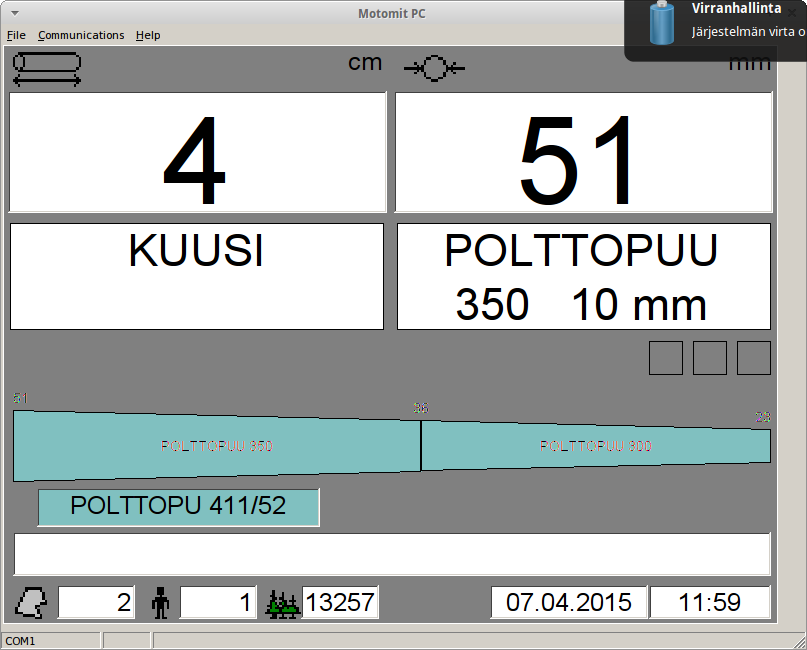
\includegraphics[width=1.00\hsize]{motomit_linux.png}
\caption{Motomit PC -ohjelmisto Winessä suoritettavana.}
\label{wine_motomit}
\end{figure}


\newpage

\chapter{Korvaava järjestelmä}
\label{ch:korvaava_jarjestelma}
Insinöörityössä tehtyjen tutkimusten perusteella päädyin esittämään yrittäjälle seuraavia vaihtoehtoja ajoneuvotietokoneen korvaamiseksi.

\section{Uusi ajoneuvotietokone}
Ehdotin ajoneuvotietokoneeksi Panasonic Toughbook CF-19 -tietokonetta. Toughbook CF-19 (kuva \ref{kuva_cf19}) on tabletiksi kääntyvä, täysvahvistettu kannettava tietokone, joka on suunnitteltu ääriolosuhteisiin. Se on suojattu niin, että se kestää pölyä, tärinää, iskuja ja -20 ja +60 °C:n välisen lämpötilavaihtelun. CF-19:ssä on Intel Core 2 Duo U7500 -prosessori, 4 Gb:n muisti ja 10,4":n näyttö. Laite on IP54-suojattu kuten alkuperäinen ajoneuvotietokone, ja se täyttää sähkömagneettisen yhteensopivuuden, tärinän, tiputuksen, vesi- ja pölytiiviyden, lämpötilankeston ja kosteudenkeston osalta Yhdysvaltain armeijan asettamat standardit \cite{cf19}. Tabletiksi kääntyminen mahdollistaa tietokoneen pienemmän tilanviennin tavallisiin kannettaviin verrattuna.

Valitsin Toughbook CF-19:n korvaajaksi, koska kääntyvän näytön takia sen saa noin 5 cm paksuksi, mikä mahdollistaa sen, että kyseiselle tietokoneelle voidaan toteuttaa helposti teline joko alkuperäiseen pidikkeeseen tai erillisenä kiinnityksenä. CF-19:ssa on lisäksi vakiona yksi RS-232-sarjaportti, joka on luotettavuudeltaan parempi kuin USB-pohjaiset adapterit. Tällöin Motomit PC voidaan liittää sarjaporttiin ja Terman laittaa menemään USB-adapterin kautta tulevasta sarjaportista. Vaikka Panasonic Toughbook CF-19 on melko iäkäs (julkaistu vuonna 2007) \cite{cf19}, mallia on hyvin saatavissa käytettyjen ja kunnostettujen tietokoneiden myyntiin erikoistuneista liikkeistä. Kosketusnäytön ansiosta erillistä hiirtä ei tarvita ja näppäimistöksi riittää ulkoinen näppäimistö, jonka pystyy laittamaan hakkuukoneessa sivuun normaalikäytösssä.

\begin{figure}[H]
\centering
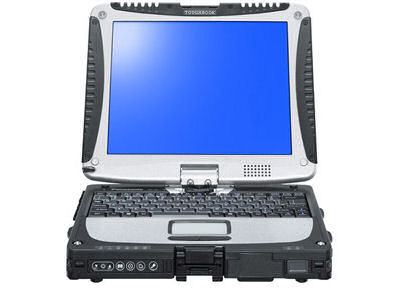
\includegraphics[width=0.50\hsize]{cf19.jpg}
\caption{Panasonic Toughbook CF-19.}
\label{kuva_cf19}
\end{figure}

\section{Uusi ajoneuvotietokone vanhaan kiinnikkeeseen}
Vaihtoehtona on myös suunnitella ja rakentaa vanhan kiinnikkeen kanssa yhteensopiva kotelo, johon asennetaan sopivan kokoinen näyttö ja esimerkiksi Raspberry Pi 2 -tietokone tai vastaava yhden kortin tietokone ja tarvittavat virtalähteet. Raspberry Pille on olemassa Dosbox- ja rpix86-ohjelmat DOS-emulointiin ja ExaGearin avulla pitäisi pystyä suorittamaan Wineä, jotta X86-ohjelmia voidaan käyttää näissä ARM-arkkitehtuurin tietokoneissa. Riittävän tehokkaita ja pieniä X86-tietokoneita on olemassa mini-ITX-standardin mukaisina versioina.

Alkuperäinen kotelo on mitattu huollon yhteydessä, jotta uutta koteloa voisi harkita. Uusi kotelo antaa enemmän liikkumavaraa osien koolle ja sijoittelulle, mutta vaatii tarkempaa suunnittelua ja sovittelua. Kotelosta suunnitellaan 3D-malli, joka sitten voidaan 3D-tulostaa (tai tulostuttaa). Kotelon mitat ovat sen verran suuria, että osien suoratulostus ei taida olla kuluttajalaitteilla mahdollista, mikä tulee ottaa huomioon 3D-mallia suunnitellessa. Myös pöly- ja kosteudenkesto tulee huomioida suunnittelussa ja toteutuksessa.

Vaihtoehtona on myös rakentaa valmiille kannettavalle yhteensopiva kiinnityslaite, jolloin vältytään mahdollisilta itse kootun järjestelmän kosteus- ja pölyongelmilta. Kiinnityslaitteen suunnittelu vaatii tiedon käytettävän tietokoneen mitoista, mutta valmistus on samantapainen kuin uudella kotelolla: 3D-mallin suunnittelu ja tulostus. Koska kotelon tulee olla varsinkin näytön takia riittävän suuri, voi olla helpointa tilata kotelo 3D-tulostuspalvelusta. Tulostuspalveluilla on tarjolla runsas joukko eri tulostusmateriaaleja, joista voi valita kappaleeseen sopivimman. Tulostuspalveluiden käyttö mahdollistaa isompien 3D-kappaleiden tulostuksen kuin yleisimmät harrastelijakäyttöön suunnatut 3D-tulostimet mahdollistavat \citep{3d_shapeways, 3d_ultimaker}

%Tulostaessa tulee huomioida. että pienemmissä 3D-tulostimissa käytetään pääsääntöisesti 2 eri muovityyppiä, ABS-muovia ja PLA:ta. ABS (akryylinitriilibutadieenistyreeni) on muovina jäykkää, kestävää ja kevyttä ja edullista. Sitä käytetäänkin mm. autojen muoviosissa ja Lego-palikoissa. Tulostuksessa ABS-muovin haittapuolina on tulostuksen aikainen vääntyily (jota ehkäistään lämpölevyllä) ja korkeahko sulamislämpötila. PLA (Polylaktidi) on uusiutuvista raaka-aineista tuotetuttu muovi. PLA on kovempaa kuin ABS ja se sulaa pienemmässä lämpötilassa. PLA on kuitenkin biohajoavaa, joten sen sopivuus motossa olevaan käyttöympäristöön ei ole taattua.


\section{Uusi ajoneuvotietokone vanhoihin kuoriin}
Toinen vaihtoehto on toteuttaa uusi tietokone Sunit Neron koteloon. Tämän vaihtoehdon etuna on, että se olisi varmasti yhteensopiva alkuperäisen pidikkeen kanssa. Vaihtoehto vaatii tarkan mietinnän komponenttien valinnan ja kiinnityksen osalta, jotta toteutus saadaan kestämään varsinkin lämpötilavaihteluita ja tärinää. Alkuperäinen kotelointi tarjoaa IP54-luokiteltuna riittävän suojan pölyä ja vesiroiskeita vastaan.

Toteutus on samanlainen kuin uusien kuorien tekemisessä, nyt vain sovitetaan vastaavat osat jo olemassa olevaan runkoon. Vanhan kotelon hyödyntämisessä on muutamia käytännön esteitä. Alkuperäistä konetta ei tulla ottamaan pois käytöstä, joten ainoaksi vaihtoehdoksi jää vastaavan koneen hankinta käytettynä. Koska kyseessä on kuitenkin jo 17 vuotta vanha, erityiskäyttöön suunniteltu laite, vastaavan koneen ja kotelon saatavuus on heikko ja hinta voi olla kallis suhteessa vastaavan kotelon uudelleentoteutukseen.

\newpage

\chapter{Yhteenveto}\
Insinöörityön tavoitteena oli selvittää työn kohteena olleen 17 vuotta vanhan hakkuukoneen alkuperäisen ajoneuvotietokoneen liitännät ja ohjelmistot ja tutkia mahdolliset vaihtoehdot korvata vanha, käyttöikänsä loppupäässä oleva alkuperäinen ajoneuvotietokone uudemmalla, hakkuukoneen järjestelmien kanssa yhteensopivalla vaihtoehdolla. Alkuperäinen tarkoitus oli tutkia vaihtoehdot ja toteuttaa käyttökuntoon asti korvaava tietokone.

Suurimmat haasteet insinöörityössä liittyivät pääsyyn työn kohteena olevalle hakkuukoneelle. Hakkuukone oli aktiivisessa käytössä Oriveden metsissä koko insinöörityön ajan, ja vierailut koneelle saatiin lopulta järjestettyä alkuperäisen ajoneuvotietokoneen huoltojen yhteydessä. Hakkuukoneen kommunikointi ajoneuvotietokoneen kanssa osoittautui kuitenkin suhteellisen yksinkertaiseksi standardinmukaiseksi RS-232-sarjamuotoiseksi liikenteeksi.

Alkuperäistä ajoneuvotietokonetta tutkimalla ja mahdollisia vaihtoehtoja punnitsemalla päädyttiin testaamaan alkuperäisten ohjelmistojen toimivuutta yhteensopivuusrajapintojen kautta tavallisessa, useamman vuoden vanhassa Linux-käyttöjärjestelmällä varustetussa kannettavassa tietokoneessa. Testaamalla selvisi, että käytettävät alkuperäiset ohjelmistot toimivat USB-sarjaporttiadapterin ja Linuxin kautta suoritettuina. Tästä voitiin päätellä, että alkuperäinen Sunit Nero -ajoneuvotietokone on korvattavissa uudemmalla olosuhteita kestävällä ajoneuvotietokoneella tai kannettavalla tietokoneella.

Uuden tietokoneen vaatimuksina on lähinnä tarvittava olosuhteiden kesto ja tarvittavat liittimet. Hakkuukoneen järjestelmät vaativat kaksi sarjaporttiliitäntää, joilla kommunikointi hakkuukoneen ja ajoneuvotietokoneen välillä tapahtuu. Hakkuukoneen sähköjärjestelmä on 24 V, mikä tulee ottaa huomioon tietokoneen sähkönsyöttöä pohdittaessa.

Työssä saatiin totetutettua ajoneuvokoneen korvaavan tietokoneen levykuva ja suoraviivaiset asennusohjeet uudelleenasennukseen. Levykuva on Xubuntu-pohjainen Linux-käyttöjärjestelmä, johon on asennettu alkuperäiset ohjelmistot toimimaan Winen ja Dosboxin avulla. Oraclen Virtualboxia käytettiin lisäksi vararatkaisuna, jolla tarvittaessa saa suoritettua ohjelmistot alkuperäisessä Windows 98 -käyttöjärjestelmässä.

Levykuvan ja tavallisen kannettavan tietokoneen avulla saatiin testattua ohjelmistojen toimivuus ajoneuvotietokoneen kanssa. Korvaavaksi tietokoneeksi ja sen kiinnittämiseksi metsäkoneeseen on tehty selvitykset, joissa päädyttiin ehdottamaan Toughbook CF-19 -tietokonetta järkevimmäksi vaihtoehdoksi ajoneuvotietokoneeksi. Koska alkuperäinen metsäkone ajoneuvotietokoneineen on aktiivikäytössä ja metsässä suurimman osan ajasta, pystytään uusi ajoneuvotietokone saattamaan asennusvalmiiksi metsäkoneen seuraavan isomman huollon yhteydessä.


%Alkuperäinen suunnitelma valmiista ajoneuvotietokoneen korvaajasta jäi saavuttamatta, mutta projekti on saatu pisteeseen, josta on helppo jatkaa toteutukseen. Ohjelmistoista on tehty valmiit levykuvat käytettäville arkkitehtuureille ja tarvittavat osat on mietitty ja alustavasti suunniteltu.




%\lipsum[12-14]

% Parhaana vaihtoehtona pidän tällä hetkellä ajoneuvotietokoneen korvaamista Panasonic Toughbook CF-19 tietokoneella. Myös Raspberry Pi 2-pohjainen ratkaisu on harkitsemisen arvoinen.

% Suurimmat haasteet insinöörityössä liittyivät pääsyyn työn kohteena olevalle hakkuukoneelle. Hakkuukone oli aktiivisessa käytössä Oriveden metsissä koko insinöörityön ajan ja vierailut koneelle saatiin lopulta järjestettyä alkuperäisen ajoneuvotietokoneen huoltojen yhteydessä. Hakkuukoneen kommunikointi ajoneuvotietokoneen kanssa osoittautui kuitenkin yksinkertaiseksi, joten järjestyneet käyntikerrat riittivät hyvin selvittämään alkuperäisen järjestelmän toimintaa ja testaamaan mahdollisessa uudessa tietokoneessa käytettäviä ratkaisuja.

% %Muita haasteita työn toteutukselle toi hektinen arki. Tyttäreni syntyi joulukuussa vaikean raskauden päätteeksi ja mukana menossa on myös neljävuotias esikoinen. Täysipäiväisesti töitä tekevänä isänä en koe valitettavasti pystyneeni täysin antamaan insinöörityölle sen ansaitsemaa panostusta. Aion kuitenkin hyödyntää tekemääni työtä toteuttamalla uuden ajoneuvotietokoneen myös käytännössä.

% Insinöörityössä saavutettiin asetetut tavoitteet uuden tietokoneen vaatimusten ja toteutusvaihtoehtojen selvittämisestä. Tarkoitus on, että hakkuukoneeseen hankitaan vielä tämän vuoden aikana edellä mainitun suunnitelman mukaisesti uusi ajoneuvotietokone, joka voidaan ottaa käyttöön alkuperäisen ajoneuvotietokoneen hajotessa seuraavan kerran.

%Lopuksi haluaisin kiittää rakasta vaimoani Jennikaa kannustuksesta ja oikolukuavusta, poikaani Tuukkaa toimimisesta apulaisena alkuperäisen koneen huollon ja tutkimisen yhteydessä ja hakkuukoneen omistajaa Arto Saalia, joka oli suureksi avuksi kaikissa käytännön järjestelyissä.\newline


% \begin{figure}[H]
% \centering
% 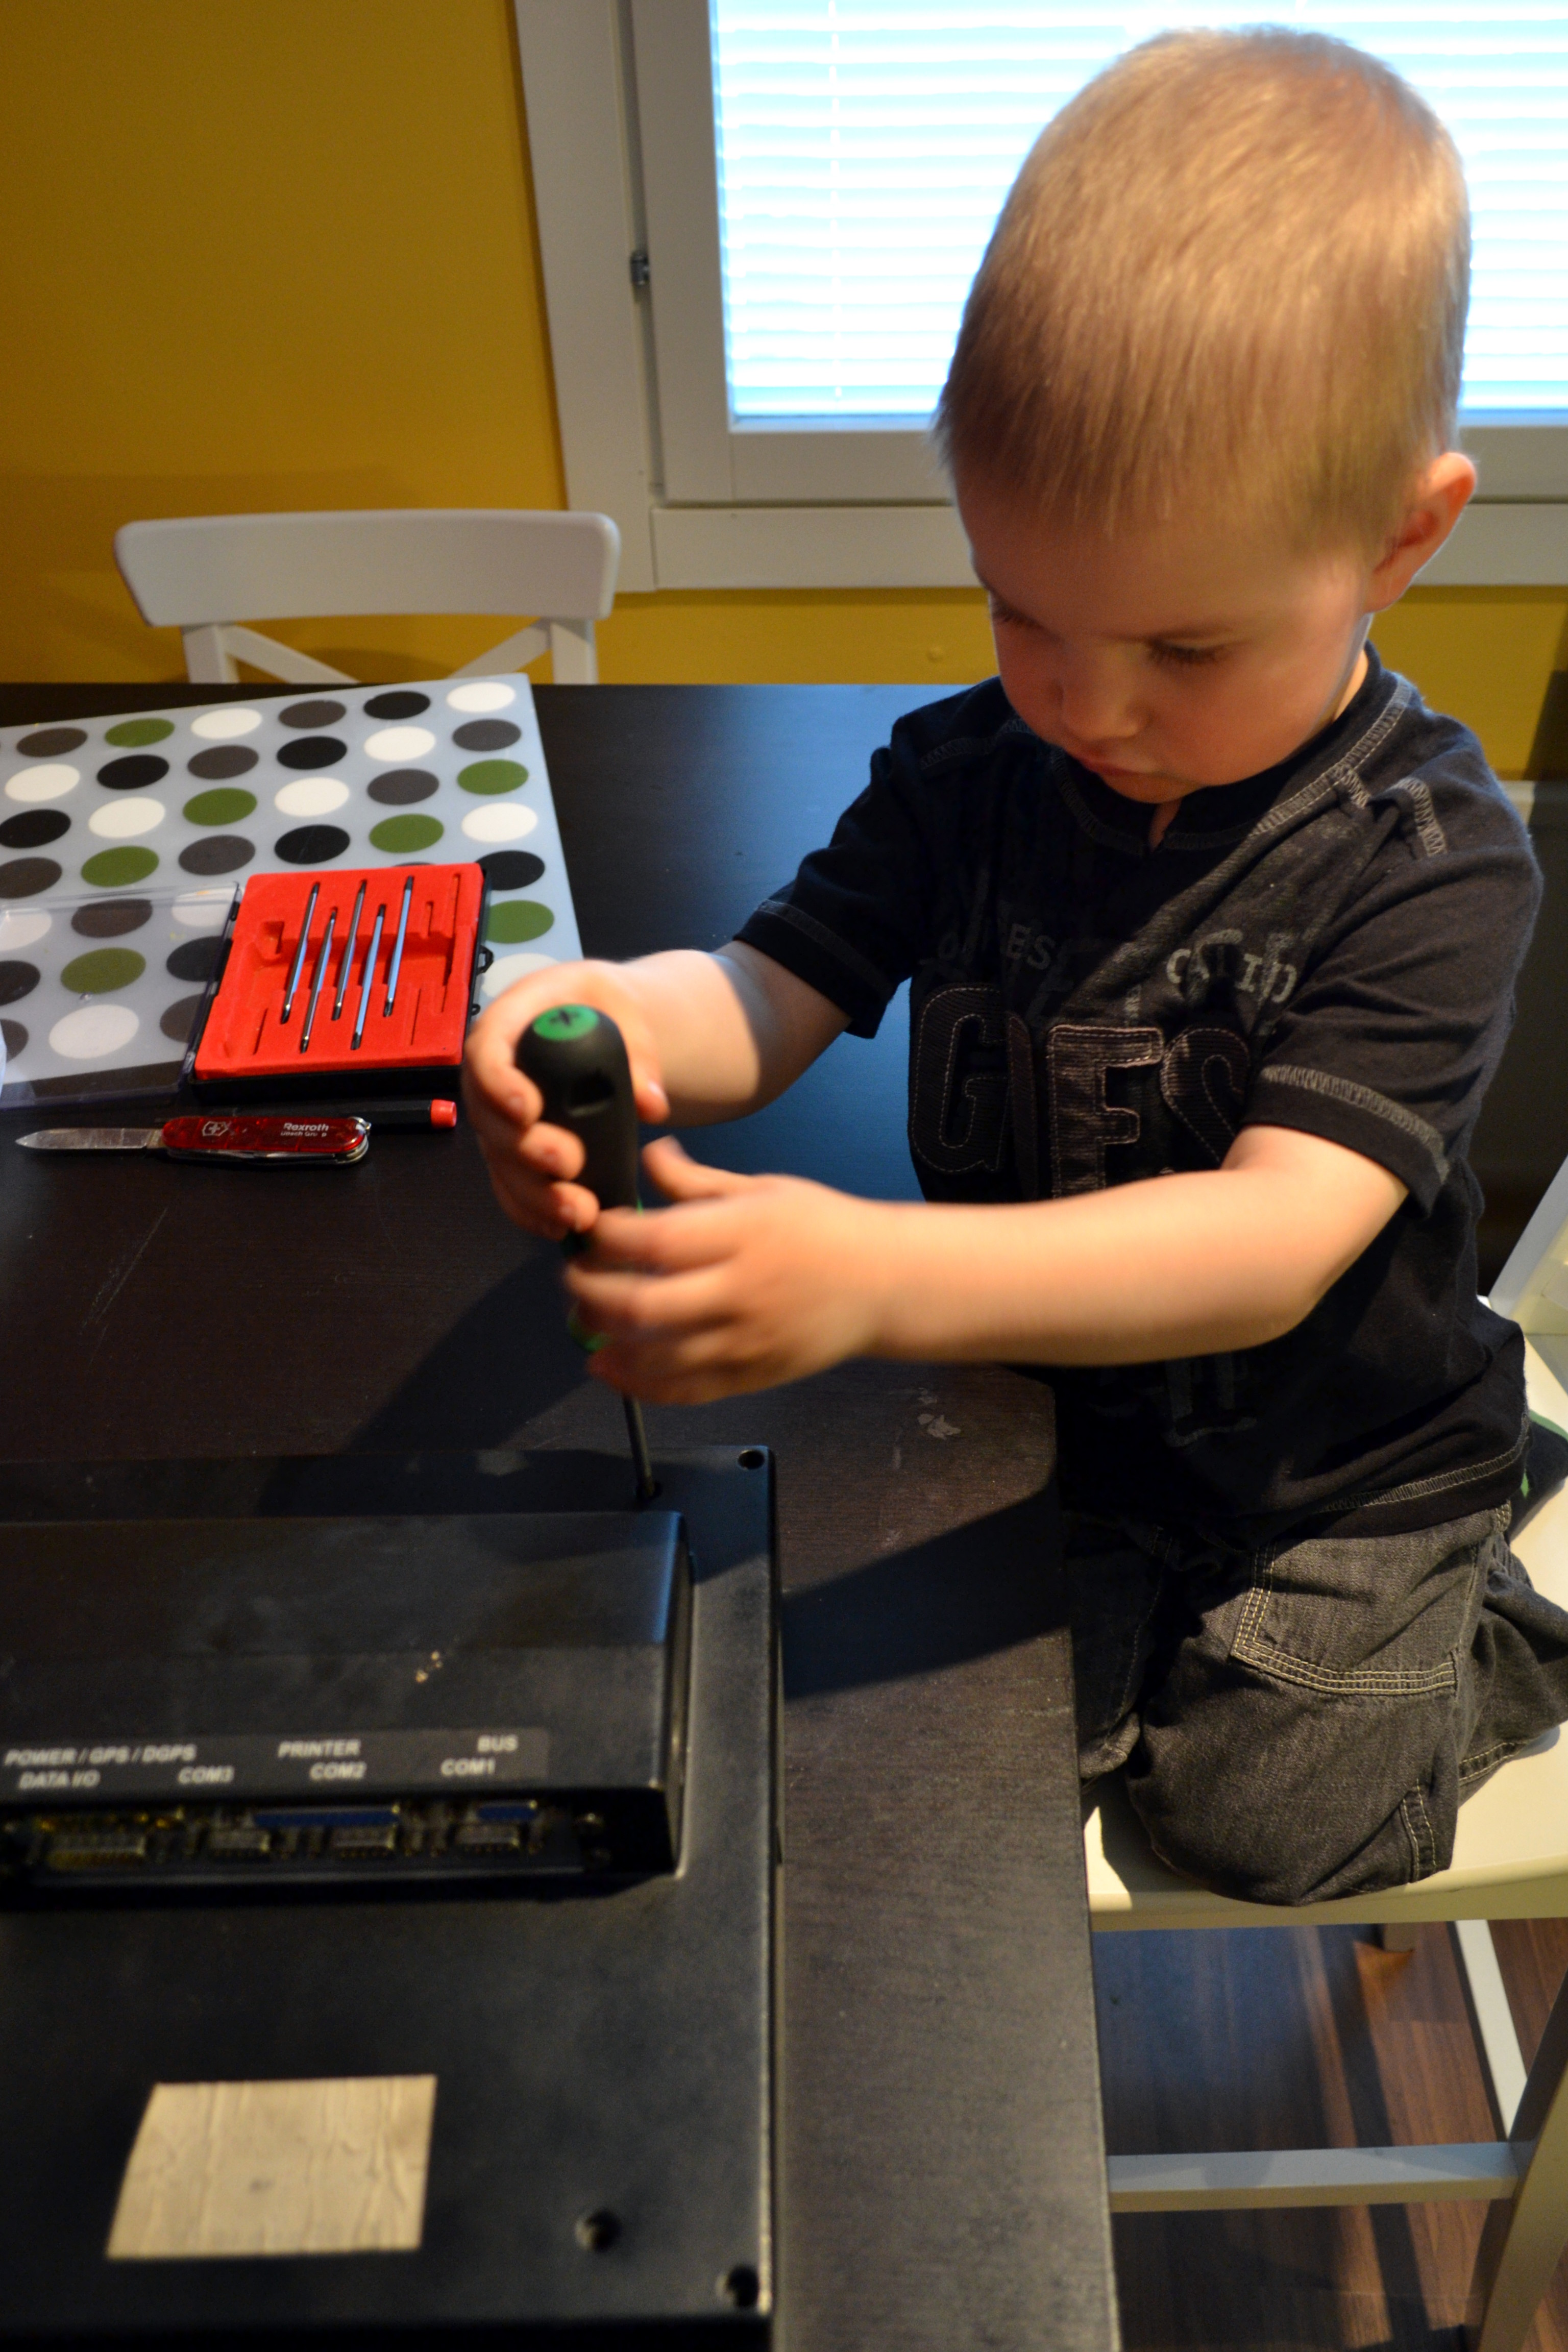
\includegraphics[width=0.80\textwidth]{tuukka_auttaa.jpg}
% \caption{Tuukka Haapaniemi valmistelemassa ajoneuvotietokoneen huoltoa}
% \end{figure}

\newpage

%----------------------------------------------------------------------------------------
%   BIBLIOGRAPHY
%----------------------------------------------------------------------------------------

\setmainfont
[BoldFont=LiberationSans-Bold.ttf,
ItalicFont=LiberationSans-Italic.ttf,
BoldItalicFont=LiberationSans-BoldItalic.ttf]
{LiberationSans-Regular.ttf}
%line space
\linespread{1}

\IfLanguageName{finnish}{\bibliographystyle{vancouver_fi}}{\bibliographystyle{vancouver}}
%line space
\singlespacing %removed otherwise the appendix are also single space
\begin{flushleft}
\begin{singlespacing}
\bibliography{motonkone_biblio}
\end{singlespacing}
\end{flushleft}

%for conting the pages
\label{LastPage}%~

%\end{document}
